\section{\texorpdfstring{Search for $T\bar{T} \to Ht$+X and \fourtop\ production}{Search for TT -> Ht+X and tttt production}}
\label{sec:HtX}
This search is focused on $\TT$ production where at least one of the $\T$ quarks decays into a Higgs boson and 
a top quark: $\TT \to HtH\bar{t}$, $HtZt$ and $HtWb$.\footnote{In the following $HtZt$ will be used to denote both $HtZ\bar{t}$ and its charge conjugate, $H\bar{t}Zt$.
Similar notation will be used for other processes, as appropriate.}
For the dominant $H\to b\bar{b}$ decay mode, the final state is \ttbar-like and contains additional heavy-flavor jets.
To a lesser extent, this search
is also sensitive to $\TT \to ZtZ\bar{t}$ and $ZtWb$, with $Z\to b\bar{b}$.

The final state is characterized by high jet and $b$-tag multiplicities, especially if both $T$ quarks decay through $T \to Ht$.
High jet and $b$-tag multiplicities are also characteristic of $\fourtop$ events, both within the SM and in BSM
extensions, which makes this search also sensitive to four-top-quark final states. 

\subsection{Event selection and categorization}

Figure~\ref{fig:shape_njet} compares the jet multiplicity distribution
after preselection between the total background and several signal scenarios. 
Signal events have, on average, higher jet multiplicity than the background.   
The higher $b$-quark content of signal events results in a higher $b$-tag multiplicity than
for the background, as illustrated in figure~\ref{fig:shape_nbtag} for events with $\geq$6 jets.

The following event selection cuts are introduced:
\begin{itemize}
  \item Given the high jet multiplicity, an additional requirement is introduced selecting events with $\geq$5 jets.
  \item In order to further reduce the non-\ttbar\ background two kinematic cuts are introduced: $\met > \unit[20]{\gev}$ and $\mtw > \unit[60]{\gev}$.

The combined effect of both cuts is $\sim \unit[90]{\%}$ efficient on the \ttbar\ background in the signal region, about $\sim \unit[95]{\%}$ on the vector-like quark signal, and reduces the non-\ttbar\ background by more than a factor of two.

  \item Several vector-like quark searches have been performed in ATLAS, one of them also in the lepton+jets channel, focusing on the decay $T\bar{T}\to Wb$+X. 
In order to ensure a non-overlapping analysis sample and to facilitate the combination of results, events accepted by the $Wb$+X search are rejected. 
This veto only removes about 2\% of the events with $\geq$6 jets and $\geq$4 $b$-tags in data.
\end{itemize}

In order to optimize the sensitivity of the search, the selected events are categorized in different channels
depending on the number of jets (5 and $\geq$6) and on the number of $b$-tagged jets (2, 3 and $\geq$4).
In addition, a further optimization can be introduced in the signal regions exploiting the features of the signal.
For high values of $m_{\T}$, the Higgs boson from the $T \to Ht$ decay is moderately boosted, and the $b\bar{b}$ pair from the Higgs boson decay has smaller angular separation than other pairs resulting from combinatorial background. In this regime, the two $b$-jets are separated enough as to be reconstructed in two individual jets but are very close in \DR.
The mass of the \bbbar\ pair with smallest \DR\ distance, $M_{bb}^{{ \rm min}\Delta R}$, provides a good approximation to the reconstructed $H\to b\bar{b}$ invariant mass, as shown in figure~\ref{fig:shape_Mbb}.

Events with $\geq$6 jets and 3 or $\geq$4 $b$-tagged jets are split into two channels each depending on the
value of the invariant mass of the two $b$-tagged jets with lowest $\Delta R$ separation: $M_{bb}^{{\rm min}\Delta R}<100\gev$ (``low $M_{bb}^{{\rm min}\Delta R}$'')
and $M_{bb}^{{\rm min}\Delta R}>100\gev$ (``high $M_{bb}^{{\rm min}\Delta R}$''). 
The high $M_{bb}^{{ \rm min}\Delta R}$ regions are enriched in 
$T\to Ht$, $H\to b\bar{b}$ decays, thus having a higher signal-to-background ratio.

A total of eight analysis channels are considered: 
(5 j, 2 b), (5 j, 3 b), (5 j, $\geq$4 b), ($\geq$6 j, 2 b), ($\geq$6 j, 3 b, low $M_{bb}^{{\rm min}\Delta R}$), 
($\geq$6 j, 3 b, high $M_{bb}^{{\rm min}\Delta R}$), ($\geq$6 j, $\geq$4 b, low $M_{bb}^{{\rm min}\Delta R}$), 
and ($\geq$6 j, $\geq$4 b, high $M_{bb}^{{\rm min}\Delta R}$), and will be used in the search.

\begin{figure}[!tb]
\centering
\begin{subfigure}{0.49\textwidth}{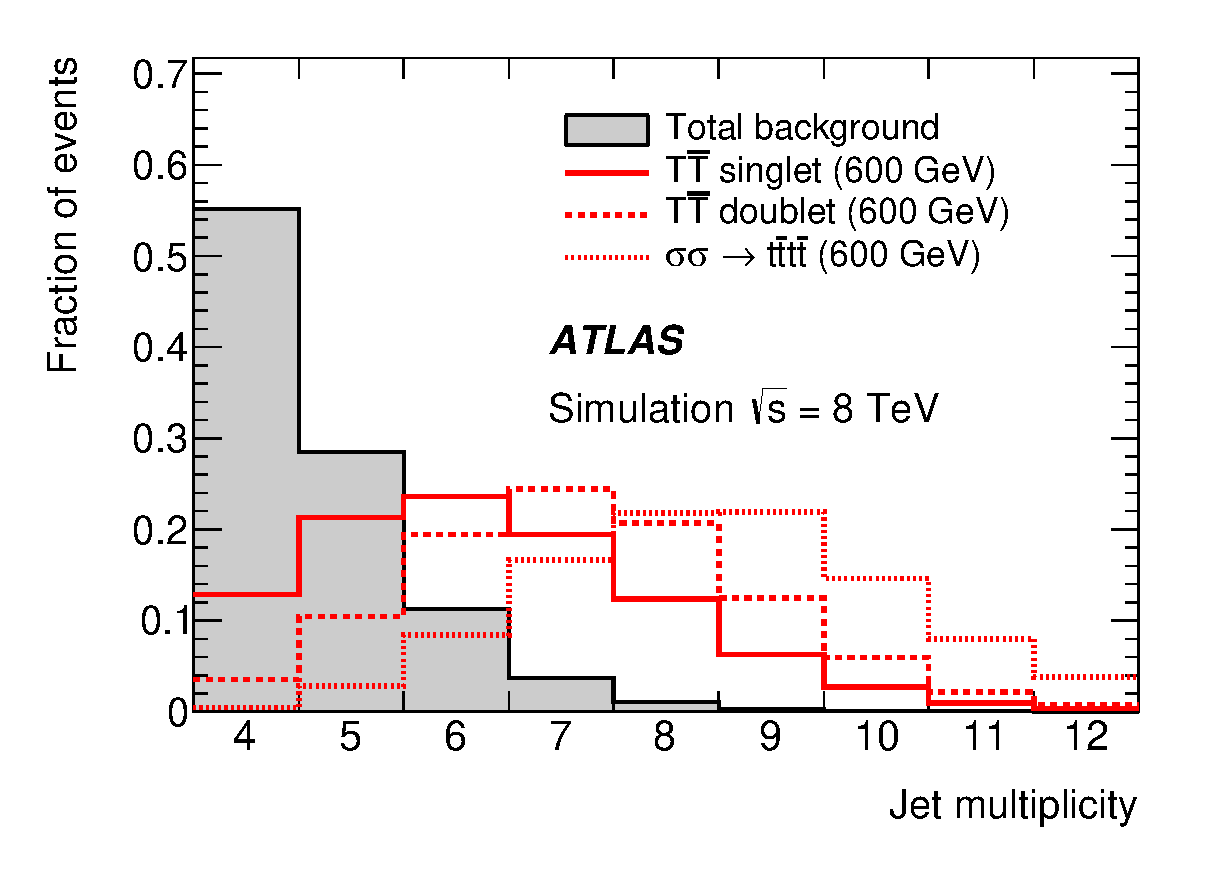
\includegraphics[width=\textwidth]{Analysis/Figures_HtX/HtXPaper/HtX/jet_n4jetin2btagin_shapes.eps}}\caption{}\label{fig:shape_njet}
    \end{subfigure}
\begin{subfigure}{0.49\textwidth}{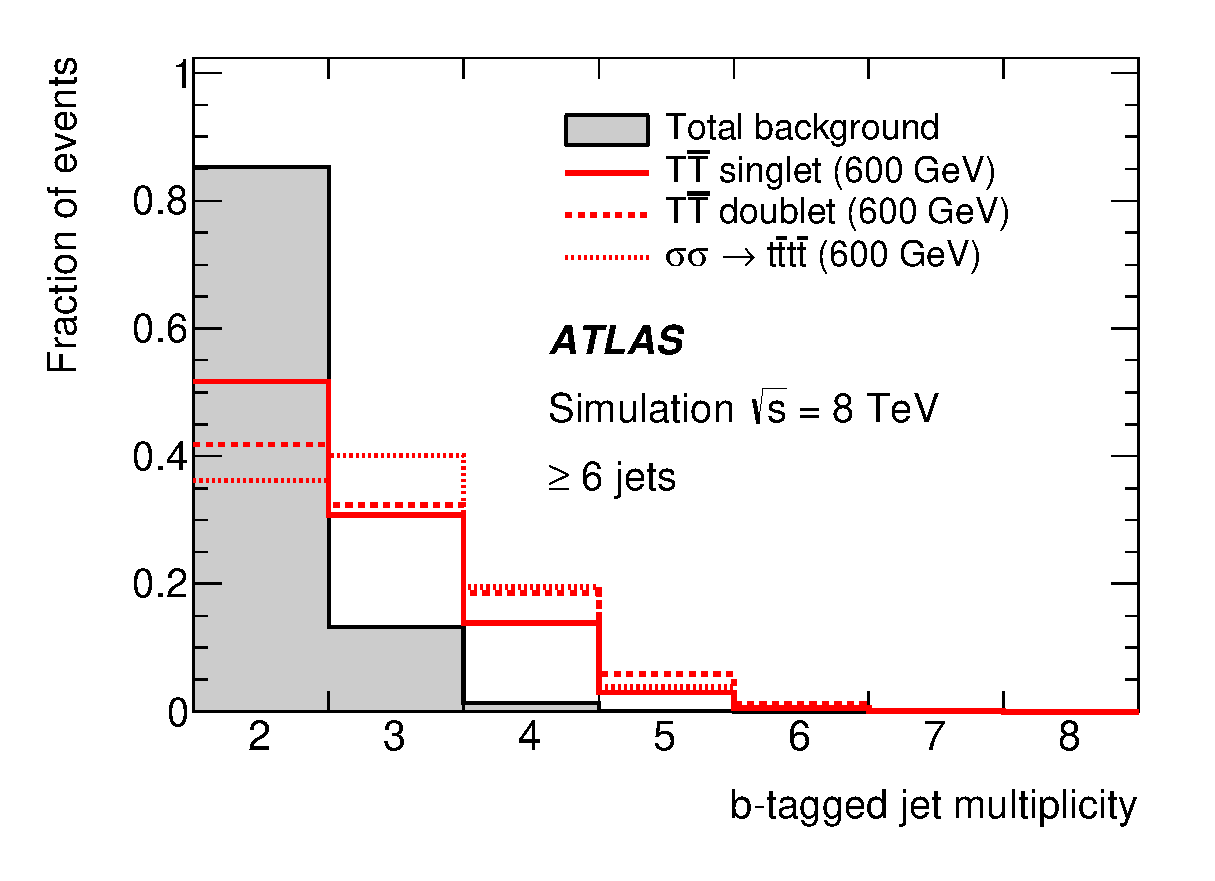
\includegraphics[width=\textwidth]{Analysis/Figures_HtX/HtXPaper/HtX/bjet_n6jetin2btagin_shapes.eps}}\caption{}\label{fig:shape_nbtag}
    \end{subfigure}
\begin{subfigure}{0.49\textwidth}{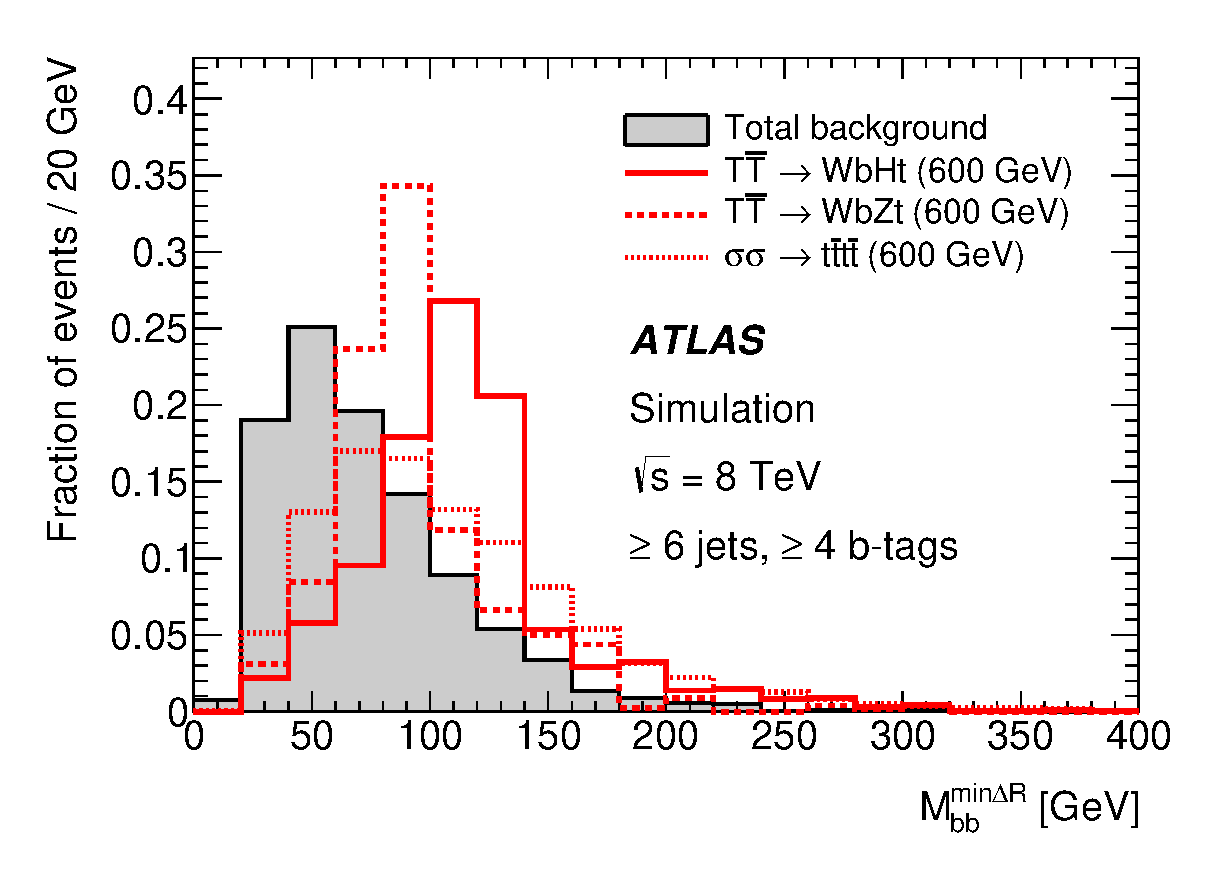
\includegraphics[width=\textwidth]{Analysis/Figures_HtX/HtXPaper/HtX/MV1_4_MinDR_bb_Mass6jetin4btagin_shapes.eps}}\caption{}\label{fig:shape_Mbb}
    \end{subfigure}
\begin{subfigure}{0.49\textwidth}{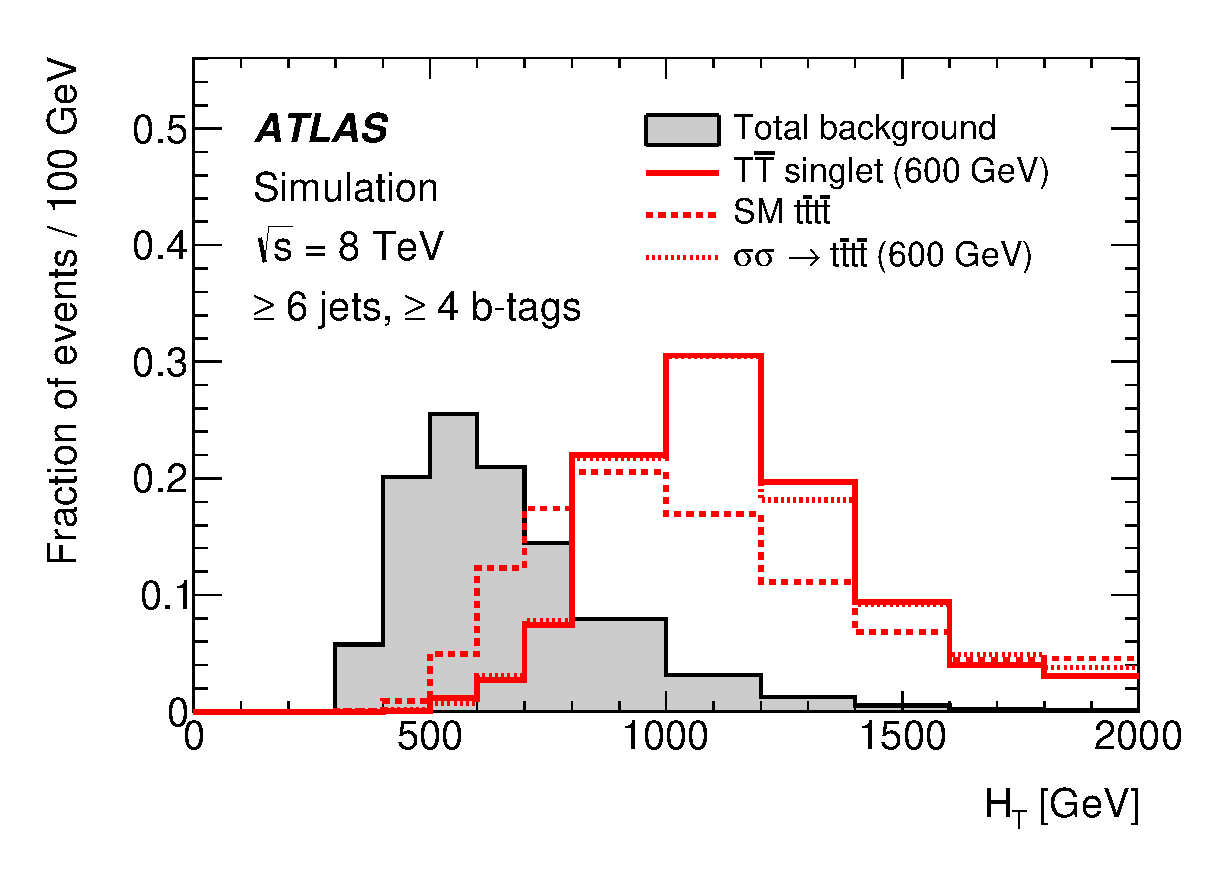
\includegraphics[width=\textwidth]{Analysis/Figures_HtX/HtXPaper/HtX/HTAll6jetin4btagin_4top_shapes}}\caption{}\label{fig:shape_HTAll}
    \end{subfigure}
\caption{Comparison of (a) the jet multiplicity distribution after preselection, (b) the $b$-tag multiplicity distribution 
  after the requirement of $\geq$6 jets, (c)  invariant mass of the two $b$-tagged jets with lowest $\Delta R$ separation, $M_{bb}^{ {\rm min}\Delta R}$,
  and (d) scalar sum of the transverse momenta of the lepton, the selected jets and the missing transverse momentum, $\HT$.
  The selection used in both (c) and (d) corresponds to events satisfying the preselection requirements and with $\geq$6 jets and $\geq$4 $b$-tagged jets.
  The distributions are compared between the total background (shaded histogram) and several signal scenarios (red solid, dashed or dotted) considered in this search:
  $\TT$ production with different decays, sgluon pair production giving a four-top-quark final state and SM $\fourtop$ production. A mass of $600\gev$ is assumed for the $\T$ quark and the sgluon.
}
\label{fig:shapes}
\end{figure}

\subsection{Discriminant variable: $\HT$}
To further improve the separation between signal and background,
the distinct kinematic features of the signal can be exploited. In particular, the large $\T$ quark mass results
in energetic leptons and jets in the final state. The variable $\HT$, defined as the scalar sum of the lepton \pT, \met\ and the \pT\ of the selected jets,
provides a suitable discriminating variable between signal and background.
Figure~\ref{fig:shape_HTAll} compares the $\HT$ distribution between signal and 
background for events with $\geq$6 jets and $\geq$4 $b$-tagged jets. 
The $\HT$ distribution peaks at $2m_T$ for signal events and is quite similar for 
different signal scenarios corresponding to pair production of exotic particles with
the same mass ($600\gev$ in this case), and significantly different from that of the background.
The discrimination between signal and background becomes better with increasing masses.

Figures~\ref{fig:prefit_HtX_unblinded_1} and~\ref{fig:prefit_HtX_unblinded_2} show the comparison of data and prediction for the $\HT$ distributions in each of the analysis
channels considered. The corresponding predicted and observed yields per channel can be found in table~\ref{tab:Prefit_Yields_HtX_unblind}.

\begin{figure}[!tp]
\begin{center}
  \begin{subfigure}{0.49\textwidth}
\includegraphics[width=\textwidth]{Analysis/Figures_HtX/HtXPaper/HtX/prefit_unblind/HTAll_5jetex2btagex8TeV.eps}
\caption{}\end{subfigure}
  \begin{subfigure}{0.49\textwidth}
\includegraphics[width=\textwidth]{Analysis/Figures_HtX/HtXPaper/HtX/prefit_unblind/HTAll_5jetex3btagex8TeV.eps}
\caption{}\end{subfigure}
  \begin{subfigure}{0.49\textwidth}
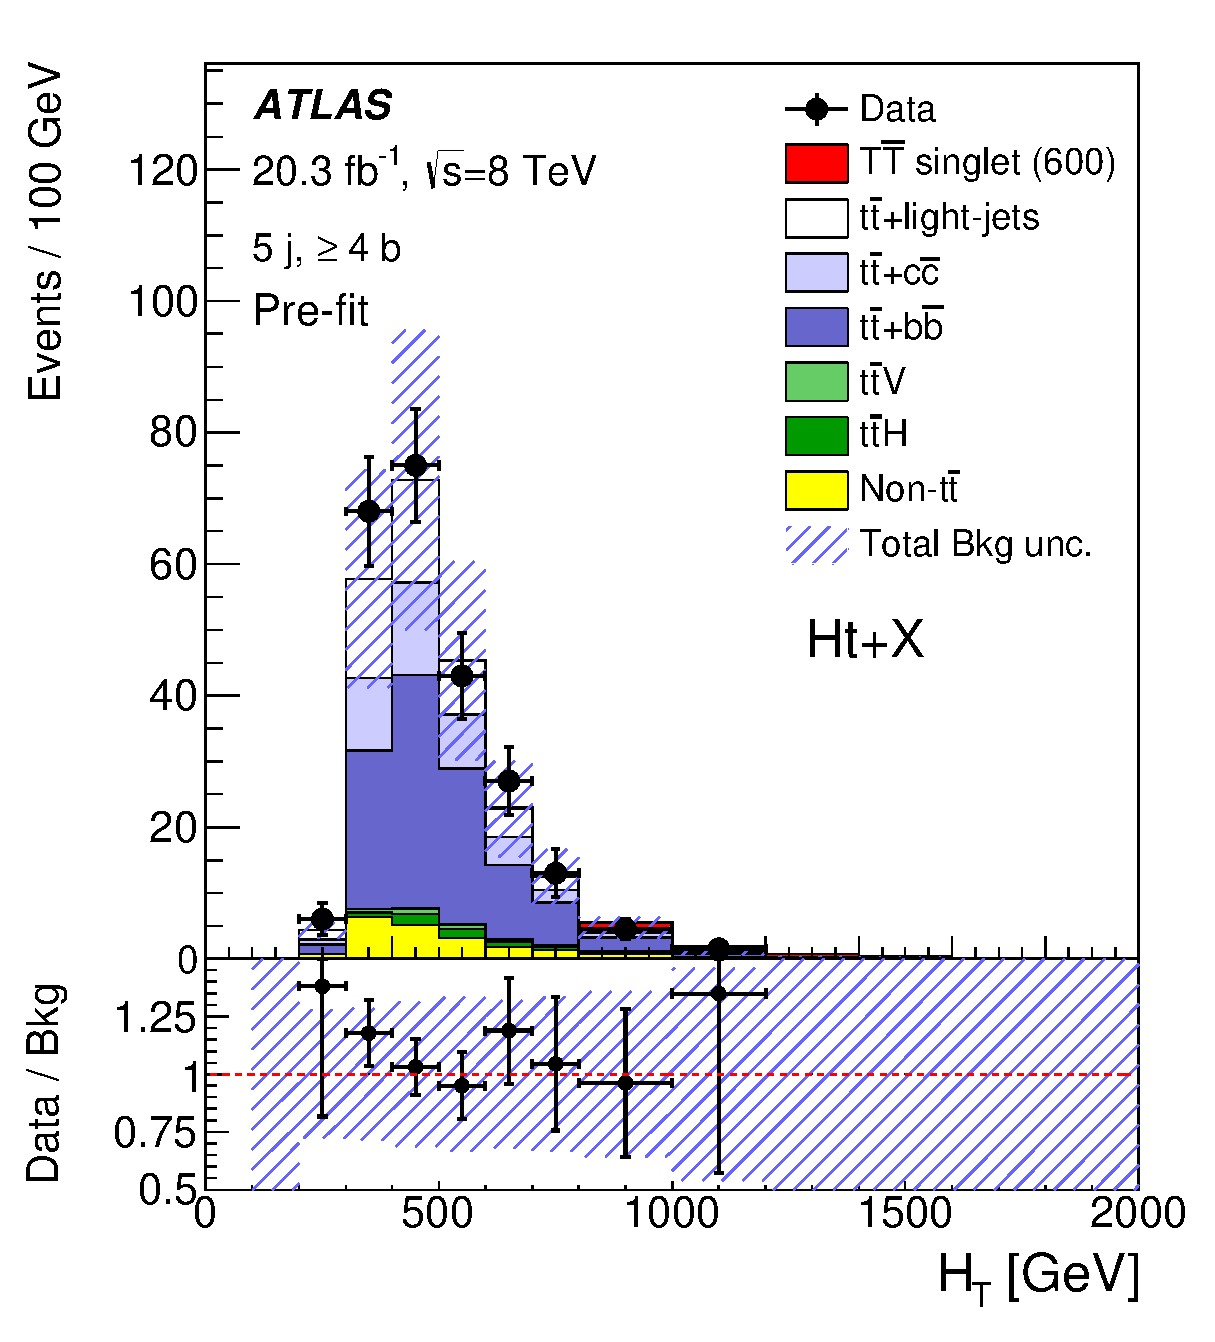
\includegraphics[width=\textwidth]{Analysis/Figures_HtX/HtXPaper/HtX/prefit_unblind/HTAll_5jetex4btagin8TeV.eps} 
\caption{}\end{subfigure}
  \begin{subfigure}{0.49\textwidth}
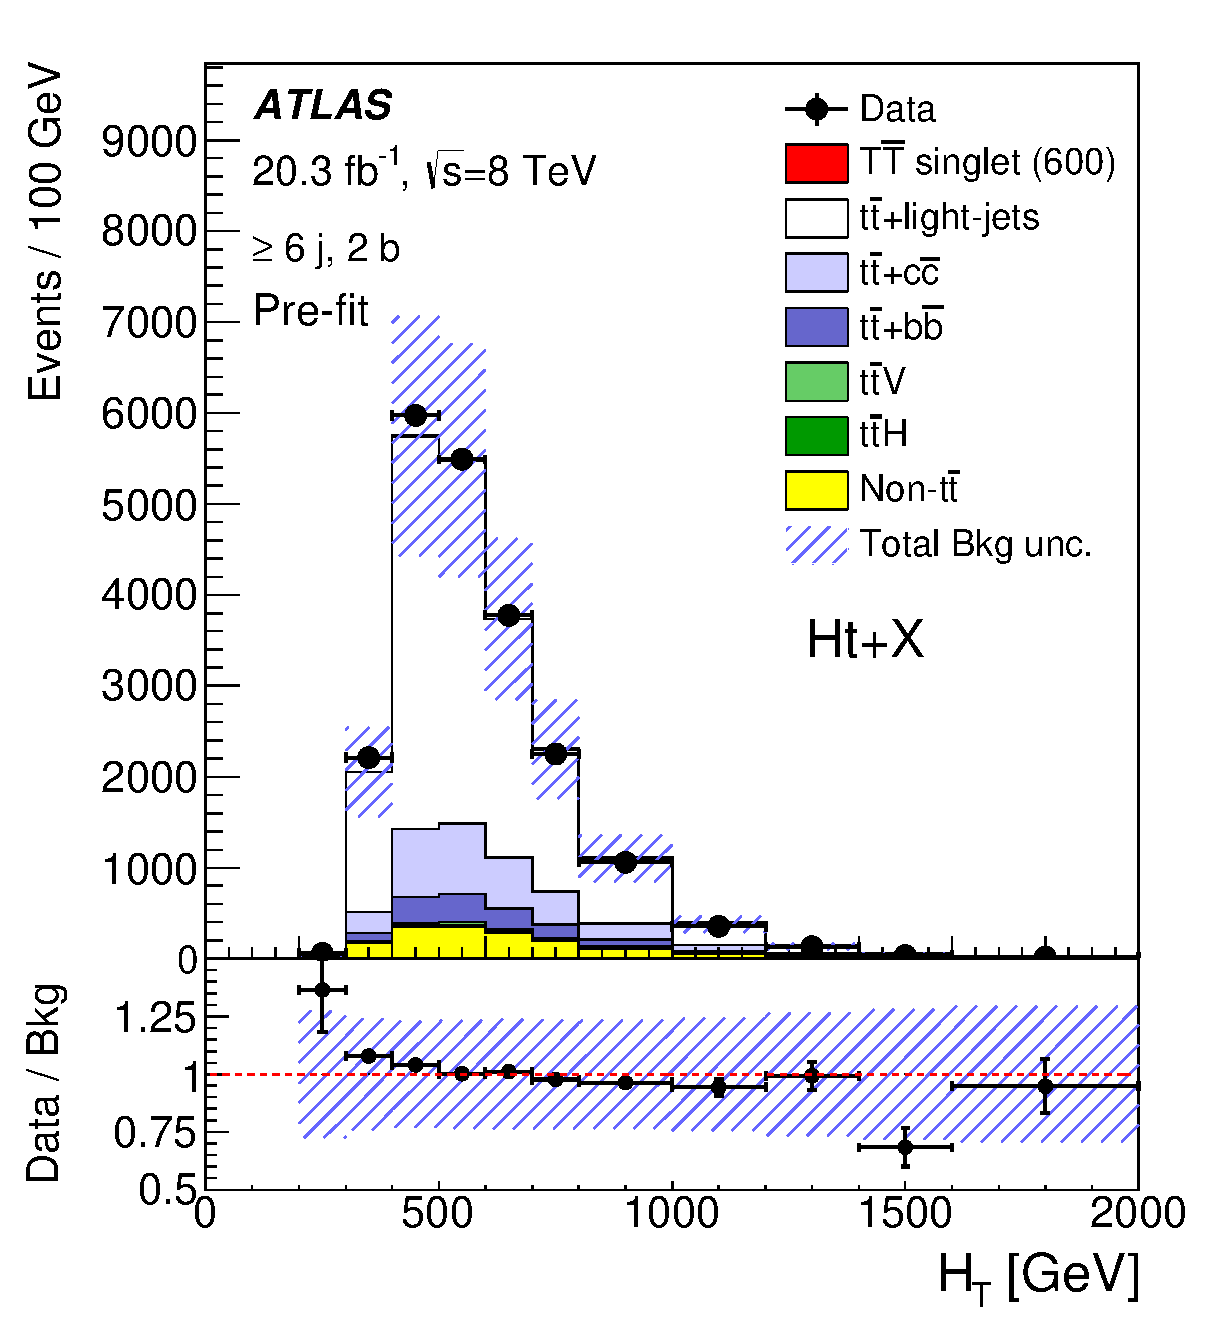
\includegraphics[width=\textwidth]{Analysis/Figures_HtX/HtXPaper/HtX/prefit_unblind/HTAll_6jetin2btagex8TeV.eps}
\caption{}\end{subfigure}
\caption{Comparison between data and prediction for the $\HT$ distribution in each of the analyzed channels:
(a) (5 j, 2 b), (b) (5 j, 3 b), (c) (5 j, $\geq$4 b), and (d) ($\geq$6 j, 2 b). 
The background prediction is shown before the fit to data. 
Also shown is the expected signal contribution from a singlet vector-like $\T$ quark with mass $m_{\T}=600\gev$.
The last bin in all figures contains the overflow and the hashed area represents the total uncertainty on the background.}
\label{fig:prefit_HtX_unblinded_1} 
\end{center}
\end{figure}
\begin{figure}[!tp]
\begin{center}
  \begin{subfigure}{0.49\textwidth}
\includegraphics[width=\textwidth]{Analysis/Figures_HtX/HtXPaper/HtX/prefit_unblind/HTAll_6jetin3btagexOutHmv18TeV.eps}
\caption{}\end{subfigure}
  \begin{subfigure}{0.49\textwidth}
\includegraphics[width=\textwidth]{Analysis/Figures_HtX/HtXPaper/HtX/prefit_unblind/HTAll_6jetin3btagexInHmv18TeV.eps}
\caption{}\end{subfigure}
  \begin{subfigure}{0.49\textwidth}
\includegraphics[width=\textwidth]{Analysis/Figures_HtX/HtXPaper/HtX/prefit_unblind/HTAll_6jetin4btaginOutHmv18TeV.eps}
\caption{}\end{subfigure}
  \begin{subfigure}{0.49\textwidth}
\includegraphics[width=\textwidth]{Analysis/Figures_HtX/HtXPaper/HtX/prefit_unblind/HTAll_6jetin4btaginInHmv18TeV.eps}
\caption{}\end{subfigure}
\caption{Comparison between data and prediction for the $\HT$ distribution in each of the analyzed channels:
(a) ($\geq$6 j, 3 b, low $M_{bb}^{{\rm min}\Delta R}$), (b) ($\geq$6 j, 3 b, high $M_{bb}^{{\rm min}\Delta R}$), 
(c) ($\geq$6 j, $\geq$4 b, low $M_{bb}^{{\rm min}\Delta R}$), and (d) ($\geq$6 j, $\geq$4 b, high $M_{bb}^{{\rm min}\Delta R}$). 
The background prediction is shown before the fit to data. 
Also shown is the expected signal contribution from a singlet vector-like $\T$ quark with mass $m_{\T}=600\gev$.
The last bin in all figures contains the overflow and the hashed area represents the total uncertainty on the background.}
\label{fig:prefit_HtX_unblinded_2} 
\end{center}
\end{figure}

\begin{table}
\footnotesize
\begin{center}
 \makebox[\textwidth][c]{
\begin{tabular}{l*{4}{c}}
\toprule\toprule
 & 5 j, 2 b & 5 j, 3 b & 5 j, $\geq$4 b & $\geq$6 j, 2 b\\
\midrule
$T\bar{T}$ ($m_{\T}=600\gev$) \\
{\,} Singlet  & $52.5 \pm 4.2$ & $19.0 \pm 2.3$ & $5.8 \pm 1.2$ & $123.3 \pm 6.2$\\
{\,} $(T,B)$ or $(X,T)$ doublet& $25.8 \pm 2.0$ & $14.0 \pm 1.4$ & $5.0 \pm 1.0$ & $154.1 \pm 6.4$\\
$\sigma\sigma \to \fourtop$ ($m_{\sigma}=800\gev$) & $2.0 \pm 0.3$ & $1.4 \pm 0.3$ & $0.3 \pm 0.1$ & $64.8 \pm 4.6$\\
$\fourtop$+X (Tier (1,1), $m_{\KK}=800\gev$) & $1.0 \pm 0.4$ & $0.6 \pm 0.3$ & $0.06 \pm 0.05$ & $180 \pm 29$\\
%SM $\fourtop$ & $0.06 \pm 0.01 $ & $0.04 \pm 0.01 $ & $0.01 \pm 0.0 $ & $0.9 \pm 0.05 $ \\ 
\midrule
$t\bar{t}$+light-jets & $32400 \pm 5300$ & $2930 \pm 520$ & $48 \pm 12$ & $16200 \pm 4000$\\
$t\bar{t}+c\bar{c}$ & $3800 \pm 2100$ & $730 \pm 410$ & $42 \pm 24$ & $3300 \pm 1800$\\
$t\bar{t}+b\bar{b}$ & $1530 \pm 800$ & $800 \pm 420$ & $108 \pm 58$ & $1300 \pm 700$\\
$t\bar{t}V$ & $140 \pm 46$ & $24.9 \pm 8.1$ & $2.9 \pm 1.0$ & $172 \pm 56$\\
$t\bar{t}H$ & $39.2 \pm 1.7$ & $20.8 \pm 1.6$ & $5.6 \pm 0.7$ & $60.2 \pm 4.5$\\
$W$+jets & $1600 \pm 1000$ & $111 \pm 71$ & $5.0 \pm 3.4$ & $770 \pm 530$\\
$Z$+jets & $360 \pm 120$ & $24.8 \pm 8.4$ & $1.2 \pm 0.5$ & $185 \pm 67$\\
Single top & $1630 \pm 320$ & $169 \pm 36$ & $7.0 \pm 1.0$ & $730 \pm 200$\\
Diboson & $85 \pm 27$ & $7.3 \pm 2.5$ & $0.4 \pm 0.2$ & $45 \pm 15$\\
Multijet & $133 \pm 48$ & $33 \pm 12$ & $6.9 \pm 2.6$ & $56 \pm 20$\\
\midrule
Total background & $41700 \pm 6400$          & $4840 \pm 900$          & $228 \pm 69$          & $22800 \pm 5200$         \\
\midrule
Data & $43319$ & $5309$ & $244$ & $23001$\\
\bottomrule\bottomrule 
\end{tabular}
} %makebox
\vspace{0.1cm}

 \makebox[\textwidth][c]{
\begin{tabular}{l*{4}{c}}
\toprule\toprule
 & \begin{tabular}{@{}c@{}}$\geq$6 j, 3 b\\ low $M_{bb}^{{\rm min}\Delta R}$\end{tabular} & \begin{tabular}{@{}c@{}}$\geq$6 j, 3 b\\ high $M_{bb}^{{\rm min}\Delta R}$\end{tabular} & \begin{tabular}{@{}c@{}}$\geq$6 j, $\geq$4 b\\ low $M_{bb}^{{\rm min}\Delta R}$\end{tabular} & \begin{tabular}{@{}c@{}}$\geq$6 j, $\geq$4  b\\ high $M_{bb}^{{\rm min}\Delta R}$\end{tabular}\\
\midrule
$T\bar{T}$ ($m_{\T}=600\gev$) \\
{\,} Singlet & $29.5 \pm 2.0$ & $44.0 \pm 3.6$ & $17.7 \pm 1.9$ & $24.1 \pm 3.7$\\
{\,} $(T,B)$ or $(X,T)$ doublet & $50.2 \pm 2.5$ & $68.9 \pm 4.1$ & $41.0 \pm 3.9$ & $53.8 \pm 7.3$\\
$\sigma\sigma \to \fourtop$ ($m_{\sigma}=800\gev$) & $22.5 \pm 1.6$ & $50.7 \pm 3.5$ & $9.3 \pm 1.0$ & $16.2 \pm 2.6$\\
$\fourtop$+X (Tier (1,1), $m_{\KK}=800\gev$) & $33.6 \pm 2.8$ & $132.5 \pm 5.9$ & $27.7 \pm 2.3$ & $75 \pm 13$\\
%Standard Model 4 tops & $0.46 \pm 0.03 $ & $0.46 \pm 0.04 $ & $0.28 \pm 0.03 $ & $0.21 \pm 0.03 $ \\ 
\midrule
$t\bar{t}$+light-jets & $1280 \pm 350$ & $440 \pm 110$ & $38 \pm 14$ & $9.3 \pm 3.9$\\
$t\bar{t}+c\bar{c}$ & $550 \pm 320$ & $220 \pm 120$ & $53 \pm 31$ & $14.7 \pm 9.0$\\
$t\bar{t}+b\bar{b}$ & $620 \pm 330$ & $250 \pm 140$ & $178 \pm 95$ & $46 \pm 25$\\
$t\bar{t}V$ & $28.7 \pm 9.2$ & $12.5 \pm 4.2$ & $6.2 \pm 2.0$ & $1.5 \pm 0.5$\\
$t\bar{t}H$ & $24.9 \pm 1.9$ & $11.6 \pm 1.3$ & $10.6 \pm 1.2$ & $4.1 \pm 0.6$\\
$W$+jets & $68 \pm 46$ & $16 \pm 10$ & $6.6 \pm 4.8$ & $0.6 \pm 0.4$\\
$Z$+jets & $15.7 \pm 6.3$ & $3.3 \pm 1.3$ & $1.6 \pm 0.6$ & $0.3 \pm 0.1$\\
Single top & $74 \pm 22$ & $32 \pm 12$ & $7.8 \pm 2.2$ & $2.1 \pm 1.3$\\
Diboson & $4.2 \pm 1.6$ & $1.2 \pm 0.5$ & $0.4 \pm 0.1$ & $0.2 \pm 0.1$\\
Multijet & $1.9 \pm 0.8$ & $4.8 \pm 2.1$ & $<0.01$ & $2.8 \pm 1.0$\\
\midrule
Total background & $2670 \pm 680$          & $990 \pm 260$          & $300 \pm 110$          & $81 \pm 30$         \\
\midrule
Data & $3015$ & $1085$ & $362$ & $84$\\
\bottomrule\bottomrule     \\
\end{tabular}
} %makebox
%%\\
\vspace{0.1cm}
\end{center}

%
\vspace{-0.5cm}
\caption{Predicted and observed yields in each of the analysis channels considered.
The background prediction is shown before the fit to data. Also shown are the signal predictions for different benchmark scenarios considered.
The quoted uncertainties are the sum in quadrature of statistical and systematic uncertainties on the yields.}
\label{tab:Prefit_Yields_HtX_unblind}
\end{table}


\subsection{Fit results}
A fit to the data  is performed in the eight analysis channels under the background-only hypothesis, and the fitted NPs are shown in figure~\ref{fig:HtX_fit}.
The corresponding correlation matrix for the
fitted NPs can be found in figure~\ref{fig:corrmat_HtX}.
As discussed in section~\ref{subsec:fit_ttH}, given the regions considered in the fit, only few NPs are expected to be pulled and somewhat 
constrained by the data.
Such discussion is also valid for this fit since the dataset and categorization is very similar.
The removal of the 4-jet channels reduces the statistical power of the fit and some of the pulls such as the ones that were present in jet flavor composition or multijet modeling are reduced.

\begin{figure}[!tp]
\begin{center}
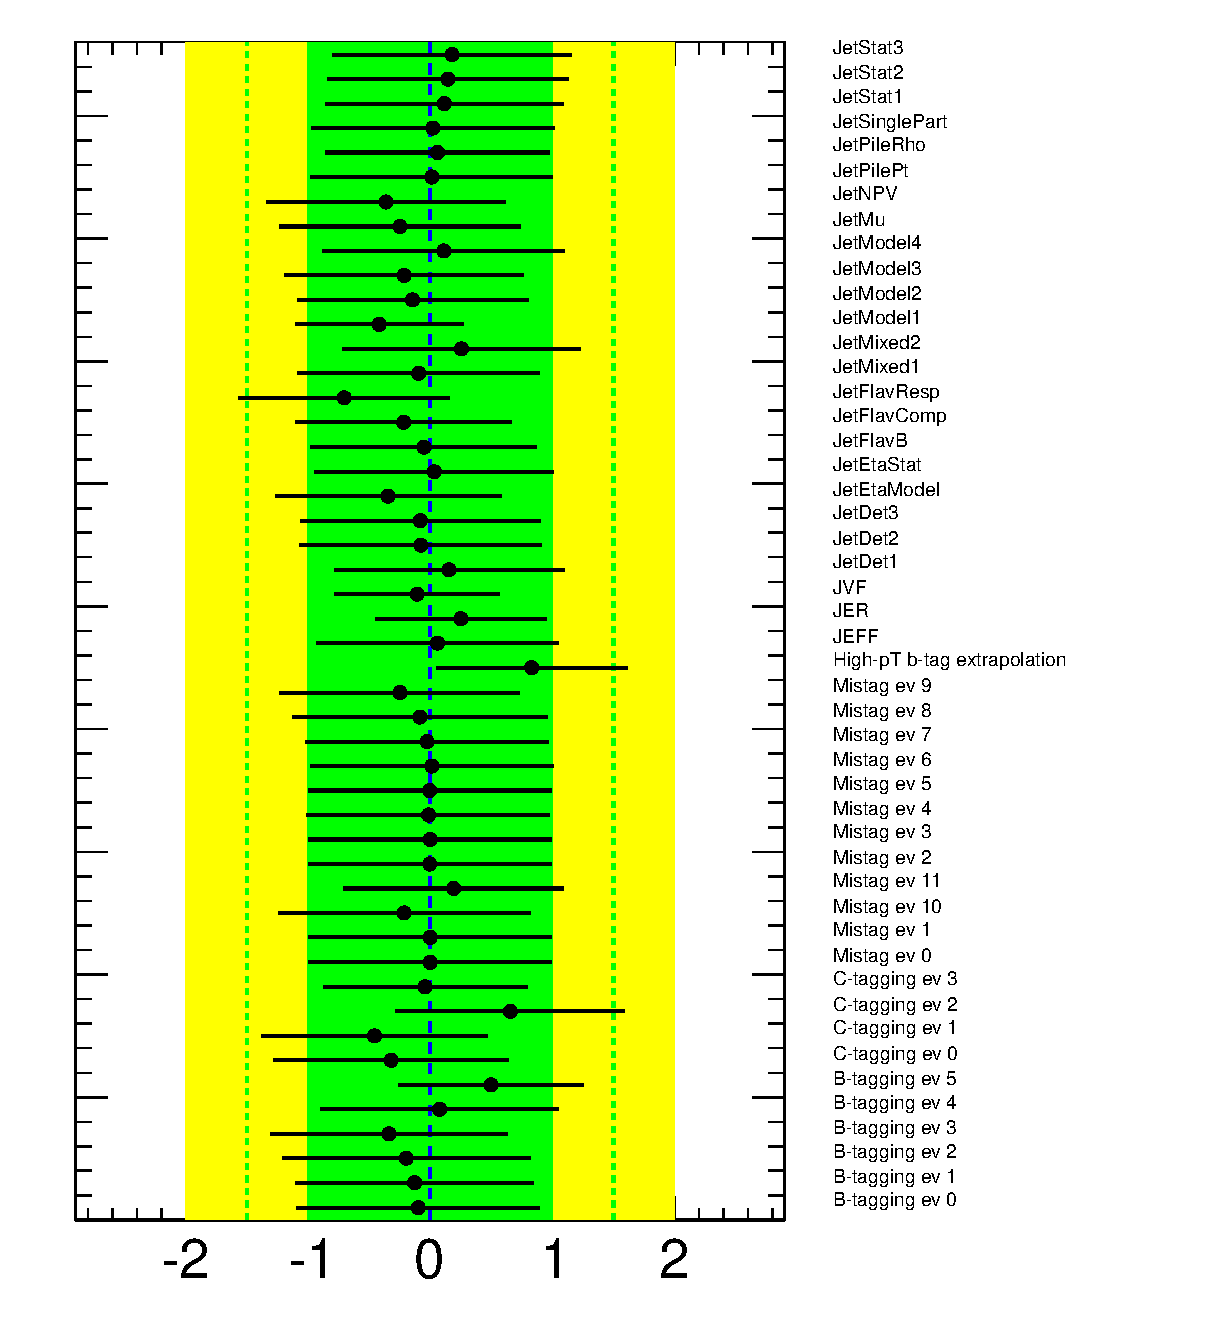
\includegraphics[trim=0cm 0cm 1.5cm 0cm, clip=true, width=0.49\textwidth]{Analysis/Figures_HtX/detectorUNC600_singlet_new.eps}
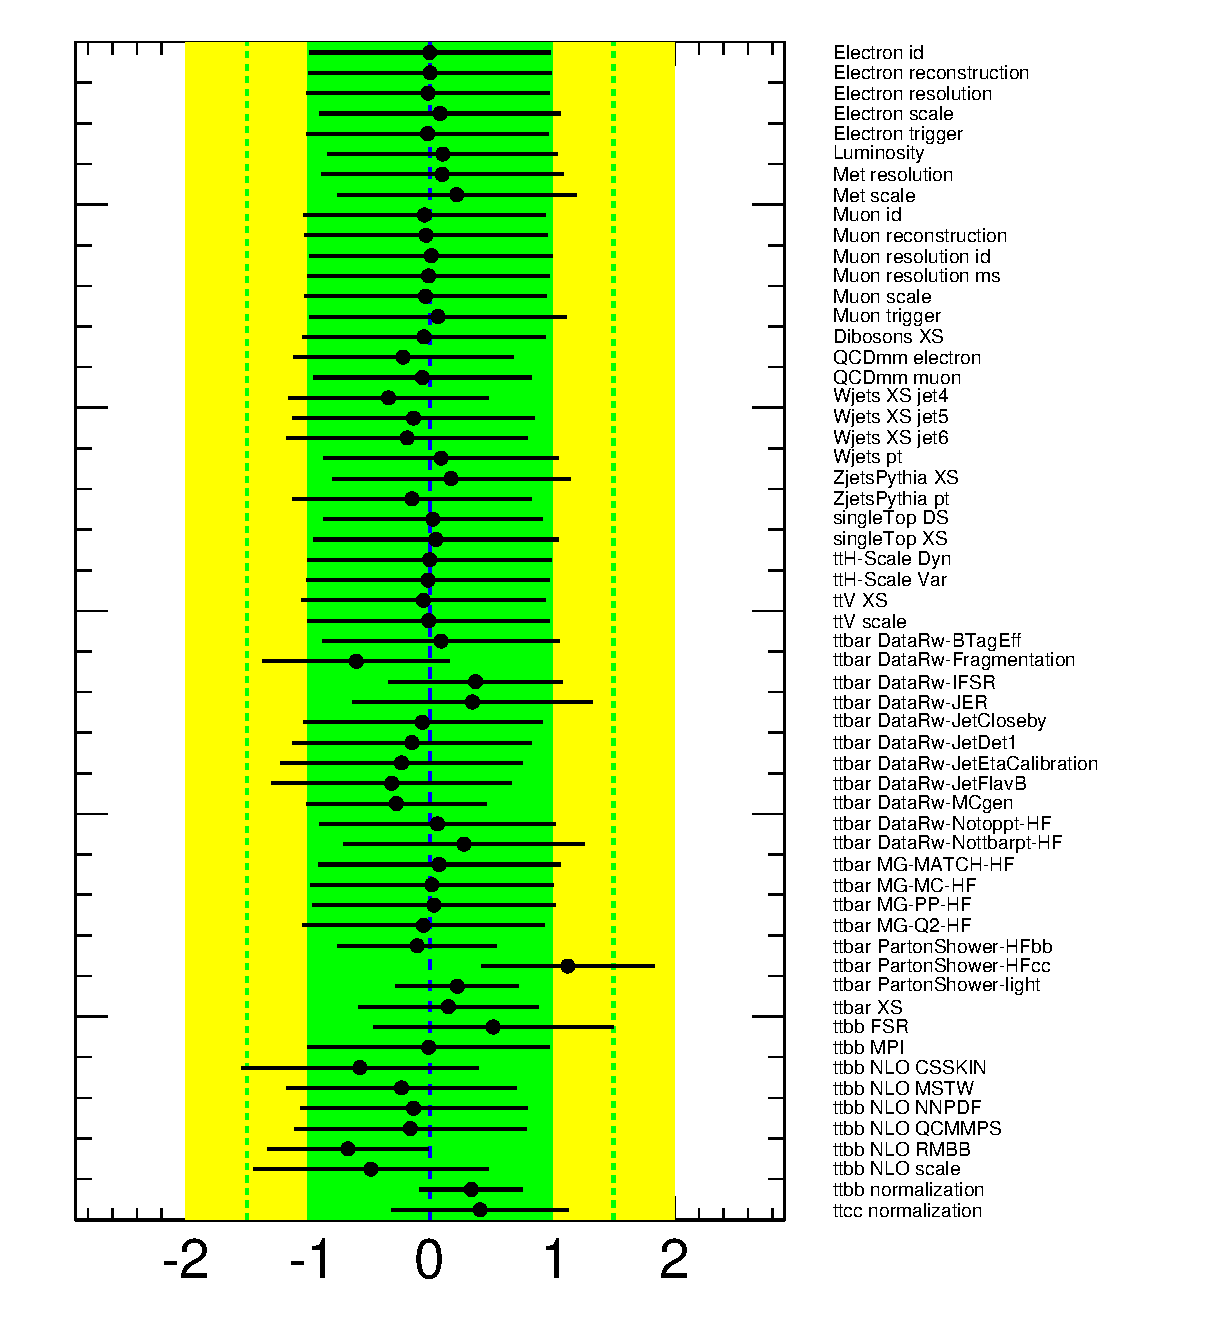
\includegraphics[trim=0cm 0cm 1.5cm 0cm, clip=true, width=0.49\textwidth]{Analysis/Figures_HtX/otherUNC600_singlet_new.eps}
\caption{Fitted NPs under the background-only hypothesis. A detailed description of the naming of the NPs can be found in appendix~\ref{app:glossary}.}
\label{fig:HtX_fit} 
\end{center}
\begin{center}
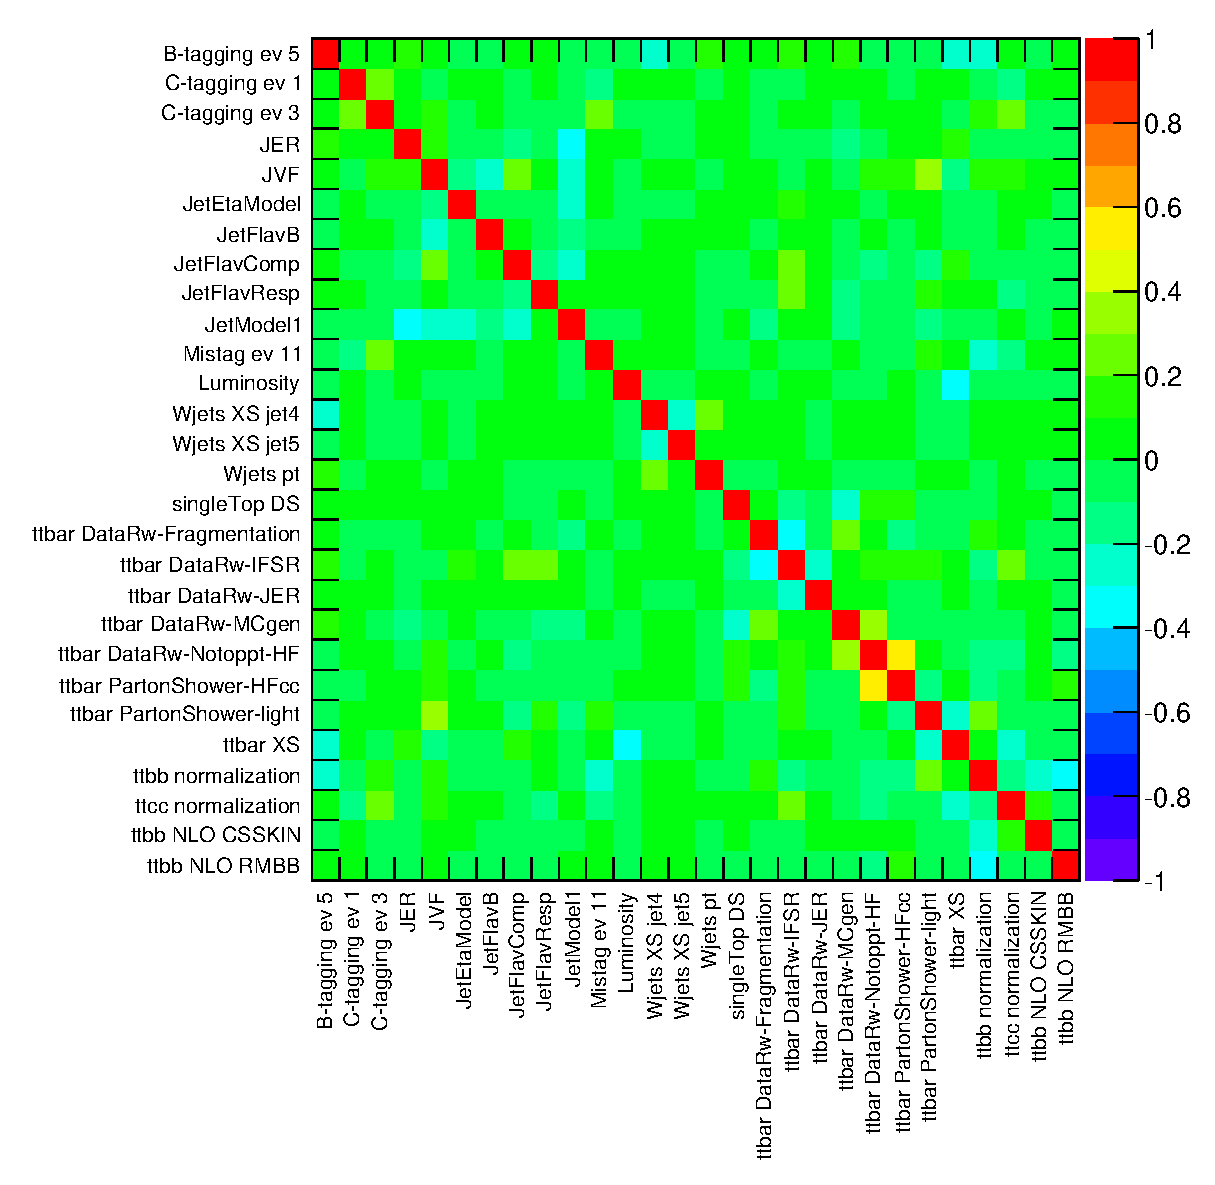
\includegraphics[width=0.6\textwidth]{Analysis/Figures_HtX/CorrMat_HtX.eps}
\caption{Correlation matrix corresponding to the fit under the background-only hypothesis.
Only NPs with a correlation coefficient of at least 20\% with any other parameter are displayed.}
\label{fig:corrmat_HtX} 
\end{center}
\end{figure}

Figures~\ref{fig:postfit_HtX_unblinded_1},~\ref{fig:postfit_HtX_unblinded_2} show the comparison of data and prediction for the $\HT$ distributions 
in each of the regions considered, after the fit to data. 
Compared to the pre-fit distributions, the total background uncertainty is significantly
reduced after the fit, not only in the background-dominated channels, but also in the signal-rich
channels, resulting in an increase in the search sensitivity. The reduced uncertainty results from the significant constraints provided by the data on some
systematic uncertainties, as well as the anti-correlations among sources of systematic uncertainty 
resulting from the fit to the data.
The corresponding post-fit yields can be found in table~\ref{tab:Postfit_Yields_HtX_unblind}.

\begin{figure}[!tp]
\begin{center}
  \begin{subfigure}{0.49\textwidth}
\includegraphics[width=\textwidth]{Analysis/Figures_HtX/HtXPaper/HtX/postfit_unblind/HTAll_5jetex2btagex8TeV.eps}
\caption{}\end{subfigure}
  \begin{subfigure}{0.49\textwidth}
\includegraphics[width=\textwidth]{Analysis/Figures_HtX/HtXPaper/HtX/postfit_unblind/HTAll_5jetex3btagex8TeV.eps}
\caption{}\end{subfigure}
  \begin{subfigure}{0.49\textwidth}
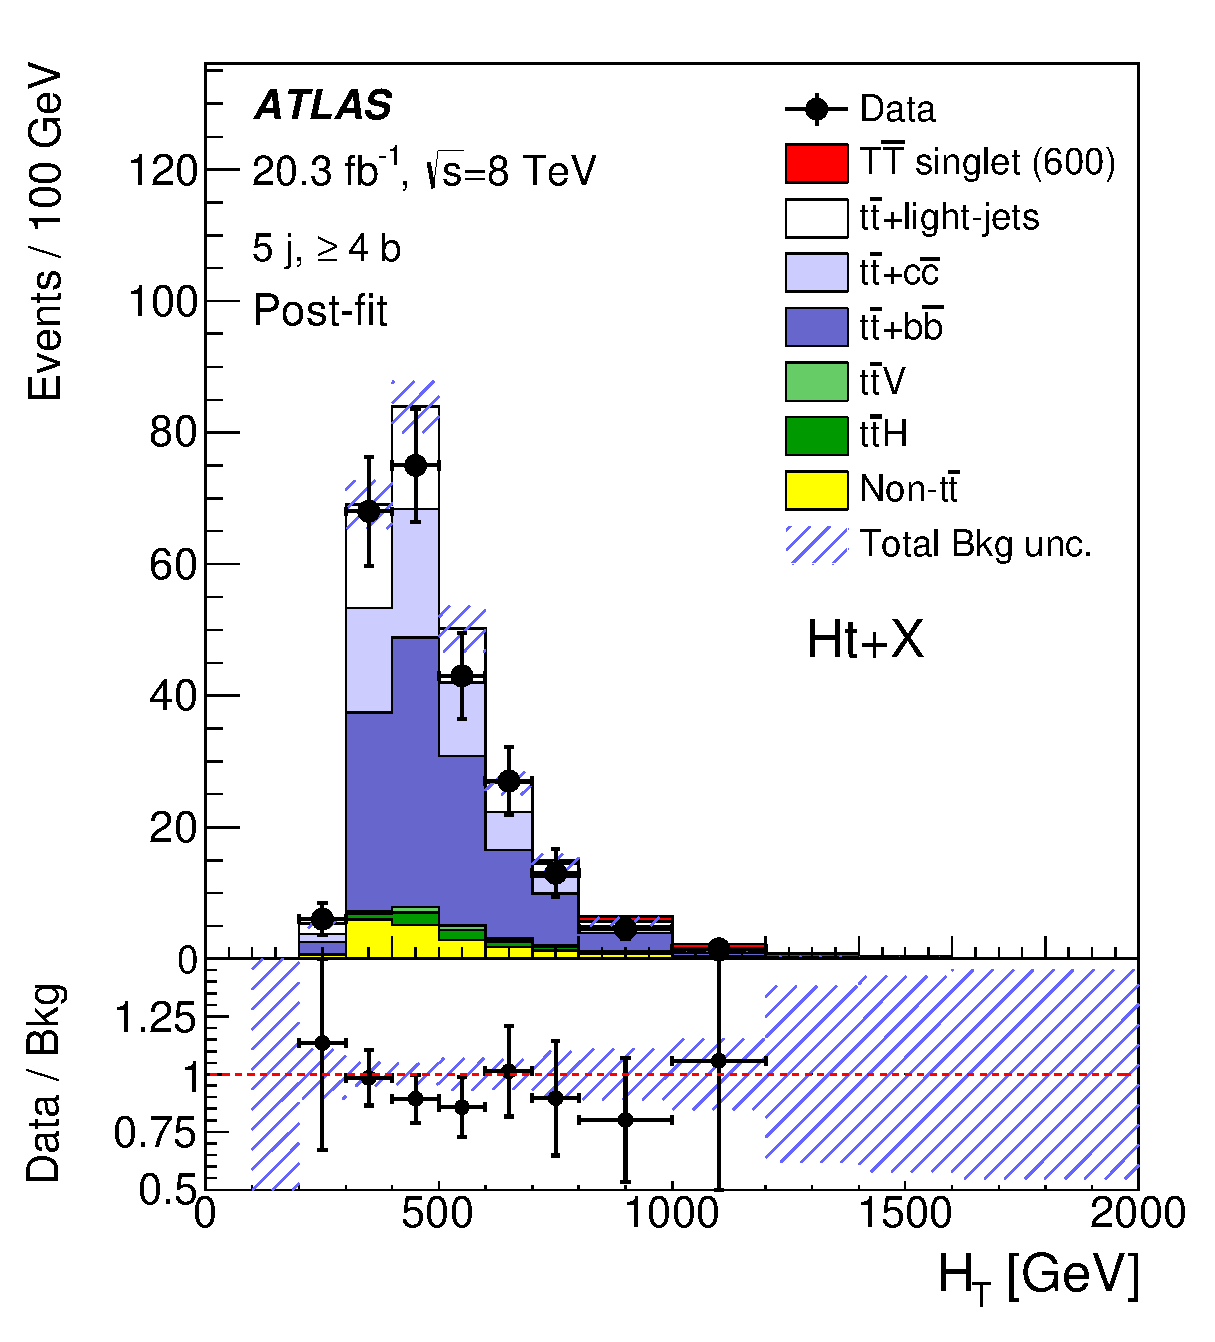
\includegraphics[width=\textwidth]{Analysis/Figures_HtX/HtXPaper/HtX/postfit_unblind/HTAll_5jetex4btagin8TeV.eps} 
\caption{}\end{subfigure}
  \begin{subfigure}{0.49\textwidth}
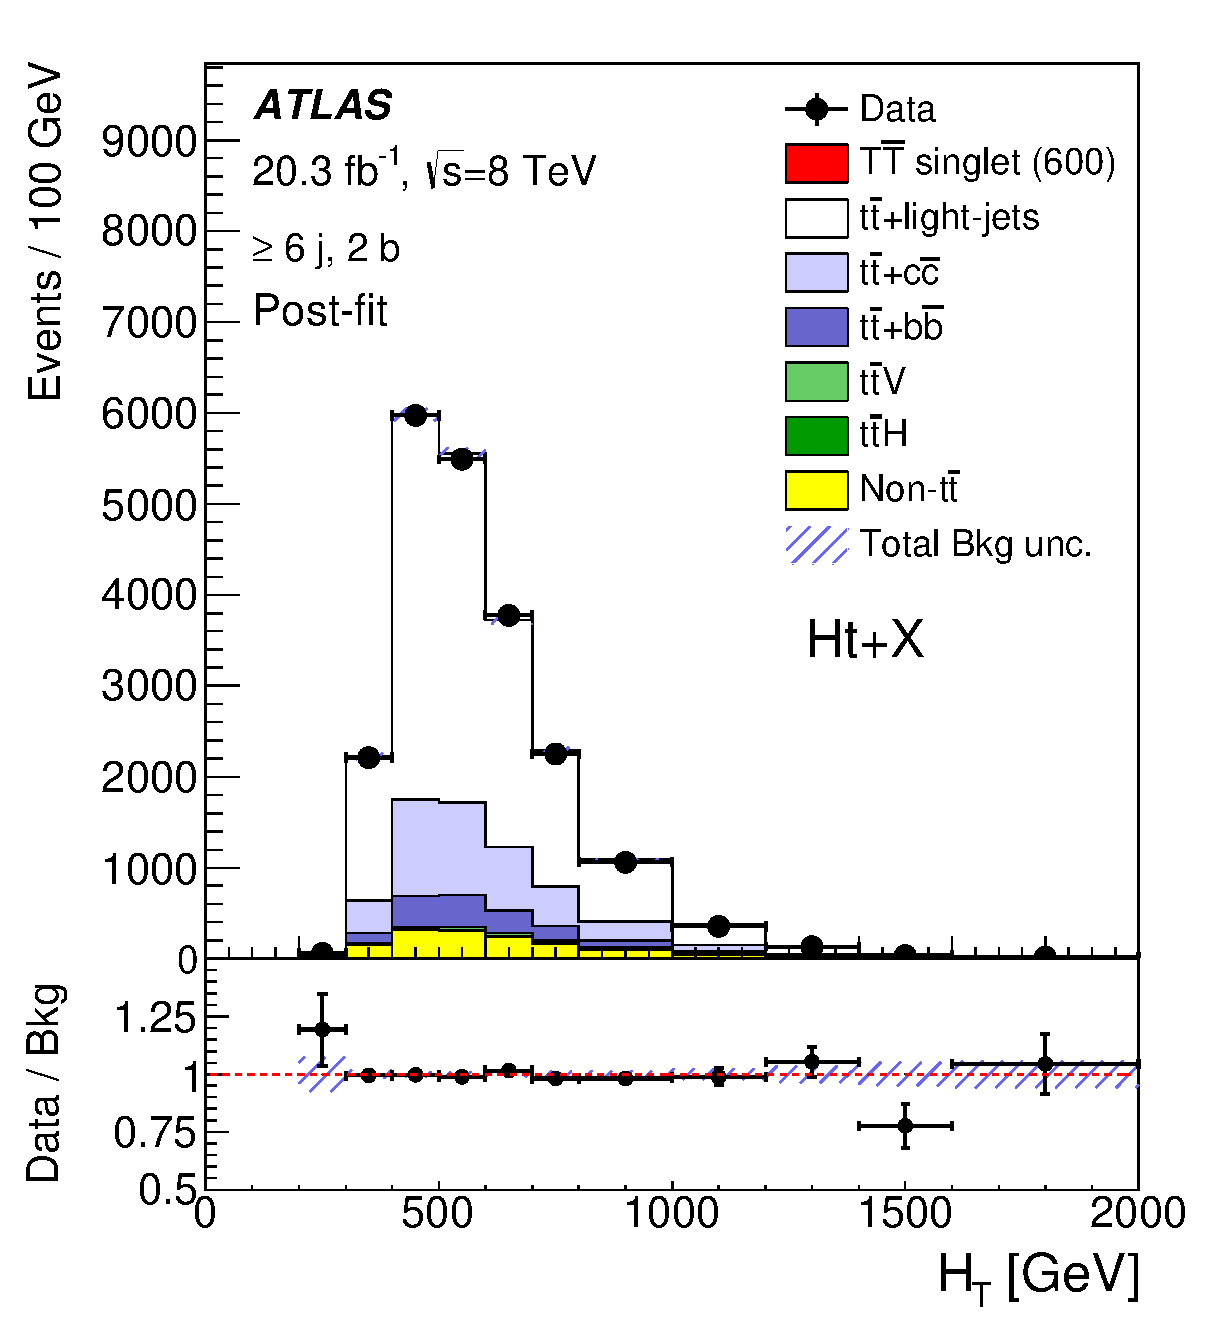
\includegraphics[width=\textwidth]{Analysis/Figures_HtX/HtXPaper/HtX/postfit_unblind/HTAll_6jetin2btagex8TeV.eps}
\caption{}\end{subfigure}
\caption{Comparison between data and prediction for the $\HT$ distribution in each of the analyzed channels:
(a) (5 j, 2 b), (b) (5 j, 3 b), (c) (5 j, $\geq$4 b), and (d) ($\geq$6 j, 2 b). 
The background prediction is shown after the fit to data. 
Also shown is the expected signal contribution from a singlet vector-like $\T$ quark with mass $m_{\T}=600\gev$.
The last bin in all figures contains the overflow and the hashed area represents the total uncertainty on the background.}
\label{fig:postfit_HtX_unblinded_1} 
\end{center}
\end{figure}

\begin{figure}[!tp]
\begin{center}
  \begin{subfigure}{0.49\textwidth}
\includegraphics[width=\textwidth]{Analysis/Figures_HtX/HtXPaper/HtX/postfit_unblind/HTAll_6jetin3btagexOutHmv18TeV.eps}
\caption{}\end{subfigure}
  \begin{subfigure}{0.49\textwidth}
\includegraphics[width=\textwidth]{Analysis/Figures_HtX/HtXPaper/HtX/postfit_unblind/HTAll_6jetin3btagexInHmv18TeV.eps}
\caption{}\end{subfigure}
  \begin{subfigure}{0.49\textwidth}
\includegraphics[width=\textwidth]{Analysis/Figures_HtX/HtXPaper/HtX/postfit_unblind/HTAll_6jetin4btaginOutHmv18TeV.eps}
\caption{}\end{subfigure}
  \begin{subfigure}{0.49\textwidth}
\includegraphics[width=\textwidth]{Analysis/Figures_HtX/HtXPaper/HtX/postfit_unblind/HTAll_6jetin4btaginInHmv18TeV.eps}
\caption{}\end{subfigure}
\caption{Comparison between data and prediction for the $\HT$ distribution in each of the analyzed channels:
(a) ($\geq$6 j, 3 b, low $M_{bb}^{{\rm min}\Delta R}$), (b) ($\geq$6 j, 3 b, high $M_{bb}^{{\rm min}\Delta R}$), 
(c) ($\geq$6 j, $\geq$4 b, low $M_{bb}^{{\rm min}\Delta R}$), and (d) ($\geq$6 j, $\geq$4 b, high $M_{bb}^{{\rm min}\Delta R}$). 
The background prediction is shown after the fit to data. 
Also shown is the expected signal contribution from a singlet vector-like $\T$ quark with mass $m_{\T}=600\gev$.
The last bin in all figures contains the overflow and the hashed area represents the total uncertainty on the background.}
\label{fig:postfit_HtX_unblinded_2} 
\end{center}
\end{figure}


\begin{table}
\begin{center}
\begin{tabular}{l*{3}{c}}
\toprule
\toprule
 & \begin{tabular}{@{}c@{}}$\geq$ 6 j, 2 b\\ $\mtw < 120\gev$\end{tabular} & \begin{tabular}{@{}c@{}}$\geq$ 6 j, 3 b\\ $\mtw<120\gev$\end{tabular} & \begin{tabular}{@{}c@{}}$\geq$ 6 j, $\geq$ 4 b\\ $\mtw < 120\gev$\end{tabular} \\

\midrule
$t\bar{t}+$light-jets &$8940 \pm 740$&$1000 \pm 130$&$29.5 \pm 7.5$\\
$t\bar{t}+c\bar{c}$&$2800 \pm 860$&$700 \pm 200$&$65 \pm 18$\\
$t\bar{t}+b\bar{b}$&$790 \pm 200$&$540 \pm 120$&$138 \pm 26$\\
$t\bar{t}V$&$93 \pm 29$&$23.6 \pm 7.4$&$4.6 \pm 1.4$\\
$t\bar{t}H$&$35.5 \pm 2.0$&$21.7 \pm 1.4$&$8.65 \pm 0.77$\\
$W$+jets &$270 \pm 160$&$30 \pm 18$&$2.2 \pm 1.4$\\
$Z$+jets &$54 \pm 20$&$5.8 \pm 2.2$&$0.53 \pm 0.28$\\
Single top &$435 \pm 46$&$65.8 \pm 8.0$&$6.5 \pm 1.1$\\
Diboson &$24.2 \pm 7.7$&$3.4 \pm 1.2$&$0.26 \pm 0.11$\\
Multijet &$8.7 \pm 3.3$&$2.4 \pm 1.0$&$0.78 \pm 0.31$\\
\midrule                                                                                           
Total background &$13500 \pm 120$&$2390 \pm 46$&$256 \pm 14$\\
\midrule                                                                                          
Data                  & $13433$                & $2411$               & $246$               \\
\bottomrule
\bottomrule
\end{tabular}
\vspace{1cm}

\begin{tabular}{l*{3}{c}}
\toprule
\toprule
 & \begin{tabular}{@{}c@{}}$\geq$ 6 j, 2 b\\ $\mtw \geq 120\gev$\end{tabular} & \begin{tabular}{@{}c@{}}$\geq$ 6 j, 3 b\\ $\mtw \geq 120\gev$\end{tabular} & \begin{tabular}{@{}c@{}}$\geq$ 6 j, $\geq$ 4 b\\ $\mtw \geq 120\gev$\end{tabular} \\
 \midrule
$t\bar{t}+$light-jets &$936 \pm 97$&$96 \pm 15$&$2.69 \pm 0.69$\\
$t\bar{t}+c\bar{c}$&$340 \pm 110$&$81 \pm 24$&$7.2 \pm 2.1$\\
$t\bar{t}+b\bar{b}$&$104 \pm 29$&$74 \pm 18$&$19.6 \pm 3.9$\\
$t\bar{t}V$&$19.3 \pm 6.0$&$4.6 \pm 1.4$&$0.83 \pm 0.27$\\
$t\bar{t}H$&$6.3 \pm 0.44$&$3.61 \pm 0.28$&$1.44 \pm 0.15$\\
$W$+jets &$30 \pm 18$&$3.1 \pm 2.0$&$0.14 \pm 0.12$\\
$Z$+jets &$13.9 \pm 5.2$&$0.96 \pm 0.4$&$0.05 \pm 0.04$\\
Single top &$47.4 \pm 7.0$&$7.1 \pm 1.6$&$0.42 \pm 0.11$\\
Diboson &$3.3 \pm 1.1$&$0.38 \pm 0.15$&$0.03 \pm 0.01$\\
Multijet &$0.00 \pm 0.00$&$0.00 \pm 0.00$&$0.00 \pm 0.00$\\
\midrule                                                                             
Total background &$1500 \pm 37$&$270 \pm 10$&$32.4 \pm 2.9$\\
\midrule                                                                            
Data                  & $1495$               & $281$              & $31$              \\
\bottomrule
\bottomrule
\end{tabular}
%%\\

%
\end{center}
\caption{
Post-fit event yields under the background-only hypothesis in each of the analysis regions.
The expected signal contributions from $\st_2\bar{\st}_2$ and $\st_1\bar{\st}_1$ production,
assuming $m_{\st_2}=500\gev$, $m_{\st_1}=300\gev$, $m_{\neut}=120\gev$ and BR$(\st_2 \to H\st_1)=1$, are also shown.
The quoted uncertainties are the sum in quadrature of the statistical and
total systematic uncertainties on the yields. 
}
\label{tab:Postfit_Yields_stop2}
\end{table}


\subsection{\texorpdfstring{Limits on $\TT$ production}{Limits on TT production}}

The consistency of the data with the background prediction is assessed by 
computing the $p_0$-value for each signal scenario considered. 
The smallest $p_0$-value found, $0.44$, is obtained for $m_{\T}=600\gev$, 
BR$(\T \to Wb)=0.0$, BR$(\T \to Ht)=0.0$, and BR$(\T \to Zt)=1.0$,
and corresponds to a local significance of $0.2$ standard deviations above the background-only prediction.

Given that no significant excess is observed, upper limits at 95\% CL on the $\TT$ production \xsec\ are set in several benchmark scenarios as a function of $m_{\T}$ and are compared to the theoretical prediction, as shown in figure~\ref{fig:limits1D_TT}. 
The resulting lower limits on $m_{\T}$ correspond to the central value of the theoretical \xsec.
The scenarios considered involve different assumptions on the decay branching ratios, which are fixed by the model under consideration: singlet or doublet.
For a vector-like singlet $\T$ quark, an observed (expected) 95\% CL limit of $m_{\T}>765\,(720)\gev$ is obtained.
For a vector-like doublet $\T$ quark the observed (expected) 95\% CL lower limit is $m_{\T}>855\,(820)\gev$.
This is the most sensitive search to date for a vector-like top partner in the singlet and doublet scenarios.

%%%%%%%%%%%%%%%
\begin{figure}[!tp]
\centering
  \begin{subfigure}{0.45\textwidth}
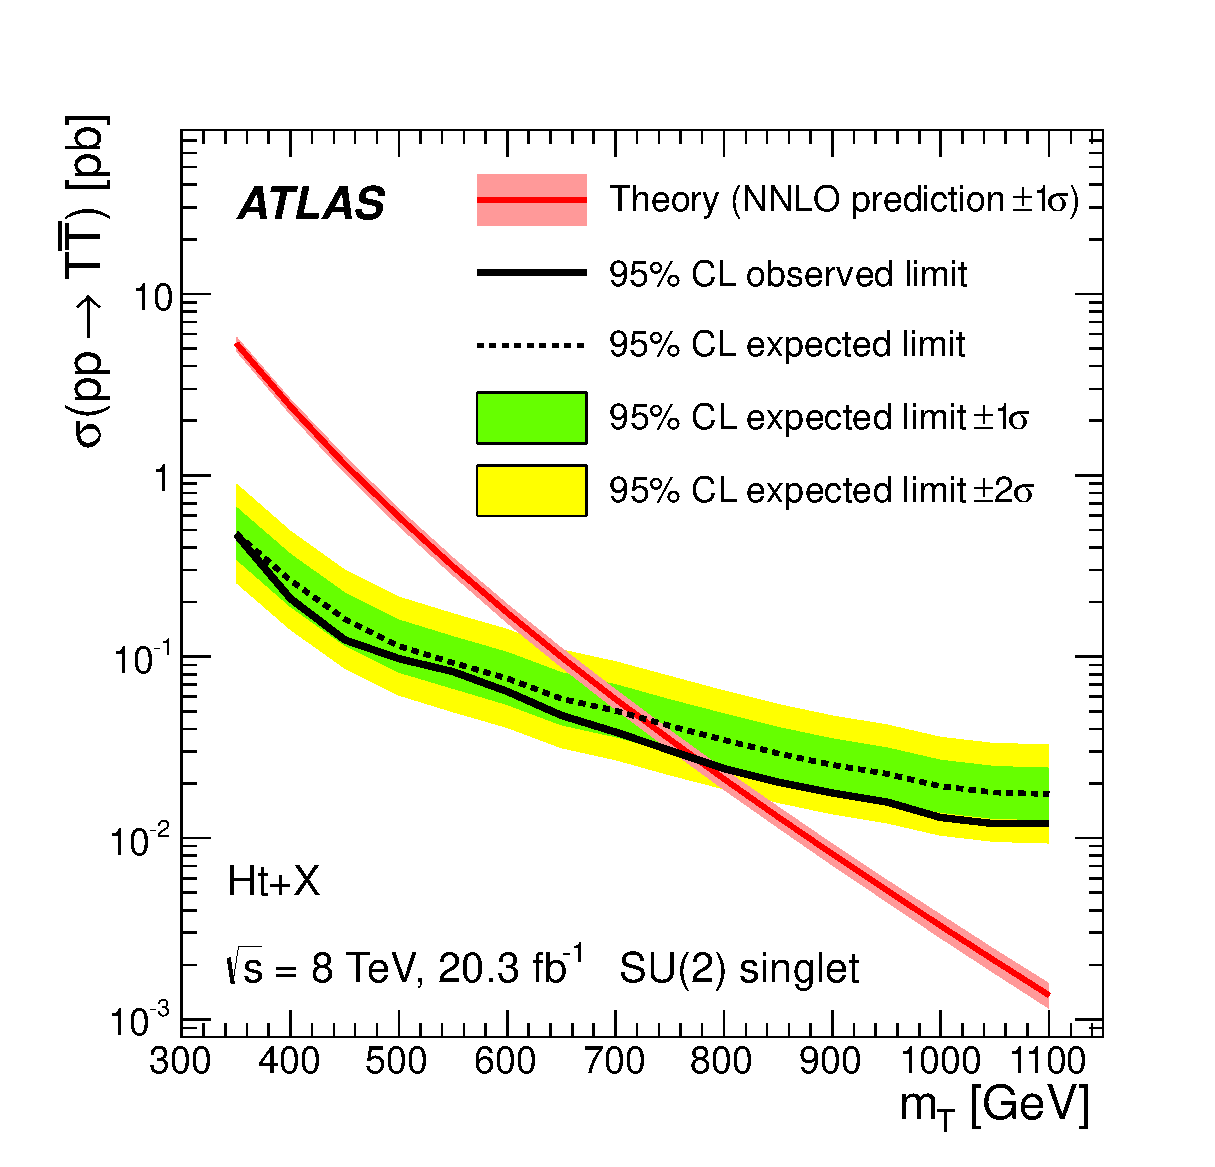
\includegraphics[width=\textwidth]{Analysis/Figures_HtX/HtXPaper/Limits/lim_HtX_singlet.eps}
\caption{}\end{subfigure}
  \begin{subfigure}{0.45\textwidth}
\includegraphics[width=\textwidth]{Analysis/Figures_HtX/HtXPaper/Limits/lim_HtX_doublet.eps}
\caption{}\end{subfigure}
\caption{Observed (solid line) and expected (dashed line) 95\% CL upper limits on the $\TT$ \xsec\ as a function of the $\T$ quark mass 
(a) for a $\T$ quark singlet, and (b) for a $\T$ quark doublet.
The surrounding shaded bands correspond to $\pm1$ and $\pm2$ standard deviations around the expected limit. 
The thin red line and band show the theoretical prediction and its $\pm1$ standard deviation uncertainty.}
\label{fig:limits1D_TT}
\end{figure}
%%%%%%%%%%%%%%%

Relaxing the assumption of a fixed branching ratio, exclusion limits can be set on vector-like $\T$ quark production for different 
values of $m_{\T}$ and as a function of the two branching ratios BR$(\T\to Wb)$ and BR$(\T\to Ht)$.\footnote{
  The branching ratio $\T\to Zt$ is determined as: BR$(\T\to Zt) = 1 - {\rm BR}(\T\to Wb) - {\rm BR}(\T\to Ht)$.
}
%To probe this branching ratio plane, the signal samples are reweighted by the ratio
%of the desired branching ratio to the original branching ratio in {\sc Protos}, and the complete analysis is repeated.
The resulting 95\% CL exclusion limits are shown in figure~\ref{fig:limits2D_TT},
for different values of $m_{\T}$.  Figure~\ref{fig:limits2D_TT_temp} presents the corresponding 
observed and expected $\T$ quark mass limits in the plane of BR$(\T \to Ht)$ versus BR$(\T \to Wb)$.
The result is an observed lower limit on the $\T$ quark mass ranging between $515\gev$ and $950\gev$  
for all possible values of the branching ratios into the three decay modes. This implies that  a $\T$ quark with mass below $515\gev$ is excluded at 95\% CL for any branching ratio configuration.
The corresponding range
of expected lower limits is between $505\gev$ and $885\gev$.
%The exclusion limits for the individual searches can be
%found in Appendix~\ref{sec:limits_appendix}. These figures illustrate the complementarity of these searches
%and how their combination improves over simply taking the most sensitive search for each assumed branching ratio scenario, 
%leading to large regions in the branching ratio plane being excluded.

\begin{figure}[!tp]
\centering
\includegraphics[width=0.9\textwidth]{Analysis/Figures_HtX/lim_2D_HtX.pdf}
\caption{
Observed (red filled area) and expected (red dashed line) 95\% CL exclusion in the plane of
BR$(\T \to Wb)$ versus BR$(\T \to Ht)$
for different values of the vector-like $\T$ quark mass.
The gray (dark shaded) area corresponds to the unphysical region where the sum of branching ratios exceeds unity. 
The default branching ratio values from the {\sc Protos} event generator for the weak-isospin singlet and doublet cases 
are shown as plain circle and star symbols respectively. 
\label{fig:limits2D_TT}}
\end{figure}

\begin{figure}[!tp]
\centering
\includegraphics[width=0.48\textwidth]{Analysis/Figures_HtX/HtXPaper/Limits/TemperaturePlots/temperature_observed_T_Ht.eps}
\includegraphics[width=0.48\textwidth]{Analysis/Figures_HtX/HtXPaper/Limits/TemperaturePlots/temperature_expected_T_Ht.eps}
\caption{Observed (left) and expected (right) limit (95\% CL) on the mass of the $\T$ quark in the plane 
of BR$(\T \to Ht)$ versus BR$(\T \to Wb)$.}
\label{fig:limits2D_TT_temp}
\end{figure}

\subsection{Analysis combination}

Several vector-like quark searches have been performed in ATLAS, one of them also in the lepton+jets channel, focusing on the decay $T\bar{T}\to Wb$+X~\cite{ATLAS-CONF-2015-012}. Given that the analyses have been designed to have non-overlapping data samples, the combination of both is straightforward and just requires the addition of the $Wb$+X search regions to the likelihood. The combined result improves respect to the individual analyses especially for the singlet mode, to which both searches are sensitive. 

  Figures~\ref{fig:limits2D_combo_TT} and~\ref{fig:limits2D_TT_temp_combo} show the observed and expected limits in the plane of BR$(\T \to Ht)$ versus BR$(\T \to Wb)$.
  The expected limits for the individual analyses are also included in order to demonstrate how the combination of the analyses improves respect to the simple overlay of the limits.
For a vector-like singlet $\T$ quark, an observed (expected) 95\% CL limit of $m_{\T}>800\,(755)\gev$ is obtained.
The limits in the branching ratio plane range between $715\gev$ and $950\gev$
for all possible values of the branching ratios into the three decay modes. This implies that any branching ratio scenario is
excluded at 95\% CL for a $\T$ quark with mass below $715\gev$. The corresponding range
of expected lower limits is between $675\gev$ and $885\gev$.

\begin{figure}[!tp]
  \begin{center}
\includegraphics[width=0.9\textwidth]{Analysis/Figures_HtX/lim_2D_combination_tesis.pdf}
\caption{
Observed (red filled area) and expected (red dashed line) 95\% CL exclusion in the plane of
BR$(\T \to Wb)$ versus BR$(\T \to Ht)$
for different values of the vector-like $\T$ quark mass for the combination of the $\TT \to Wb$+X and $\TT \to Ht$+X searches.
Also shown are the expected 95\% CL exclusion limits for the individual $Ht+X$ (blue) and $Wb+X$ (green) analyses.
The gray (dark shaded) area corresponds to the unphysical region where the sum of branching ratios exceeds unity. 
The default branching ratio values from the {\sc Protos} event generator for the weak-isospin singlet and doublet cases 
are shown as plain circle and star symbols respectively. 
\label{fig:limits2D_combo_TT}}
\end{center}
  \begin{center}
\includegraphics[width=0.48\textwidth]{Analysis/Figures_HtX/HtXPaper/Limits/TemperaturePlots/temperature_observed_T_HtWbcombination.eps}
\includegraphics[width=0.48\textwidth]{Analysis/Figures_HtX/HtXPaper/Limits/TemperaturePlots/temperature_expected_T_HtWbcombination.eps}
\caption{Observed (left) and expected (right) limit (95\% CL) on the mass of the $\T$ quark in the plane 
of BR$(\T \to Ht)$ versus BR$(\T \to Wb)$ for the combination of the $\TT \to Wb$+X and $\TT \to Ht$+X searches.}
\label{fig:limits2D_TT_temp_combo}
\end{center}
\end{figure}


\subsection{Comparison with other analyses}
In addition to the $\TT \to Wb$+X and $\TT \to Ht$+X searches, the ATLAS collaboration has performed
searches for $\TT$ production in several multilepton final states: same-sign dileptons and trileptons~\cite{Aad:2015gdg} and opposite-sign dileptons and trileptons with a $Z$ boson candidate~\cite{Aad:2014efa} (referred to as $Zb/t$+X search).
These searches have overlapping selections and thus have not been combined.  
Figure~\ref{fig:limits2D_T_Summary_temp} summarizes the most restrictive observed and expected $\T$ quark mass limits 
in the plane of BR$(\T \to Ht)$ versus BR$(\T \to Wb)$, set by any of these searches.
The observed lower limits on the $\T$ quark mass range between $730\gev$ and $950\gev$  
for all possible values of the branching ratios into the three decay modes, representing an improvement
over previous results~\cite{Chatrchyan:2013uxa}.  The corresponding range of expected lower limits is between 
$715\gev$ and $885\gev$.

\begin{figure}[!tp]
\centering
\includegraphics[width=0.48\textwidth]{Analysis/Figures_HtX/HtXPaper/Limits/TemperaturePlots/temperature_observed_T_Summary3.eps}
\includegraphics[width=0.48\textwidth]{Analysis/Figures_HtX/HtXPaper/Limits/TemperaturePlots/temperature_expected_T_Summary3.eps}
\caption{Summary of the most restrictive (a) observed and (b) expected limit (95\% CL) on the mass of the $\T$ quark 
in the plane of BR$(\T \to Ht)$ versus BR$(\T \to Wb)$  from all ATLAS searches for $\TT$ production.}
\label{fig:limits2D_T_Summary_temp}
\end{figure}

\subsection{\texorpdfstring{Limits on $\fourtop$ production}{Limits on tttt production}}

As discussed previously, this analysis is also used to set limits on four-top-quark production considering different signal benchmark
scenarios: SM-like $\fourtop$, $\fourtop$ via an EFT model with a four-top contact interaction, sgluon pair production with
decay into $t\bar{t}$, and a Universal Extra Dimension (UED) model with two extra dimensions 
compactified under the Real Projective Plane (RPP) geometry. Figure~\ref{fig:4top_data} shows the expected signal from each scenario
overlaid with the observed data in the most sensitive region.

\begin{figure}[!tbp]
  \centering
  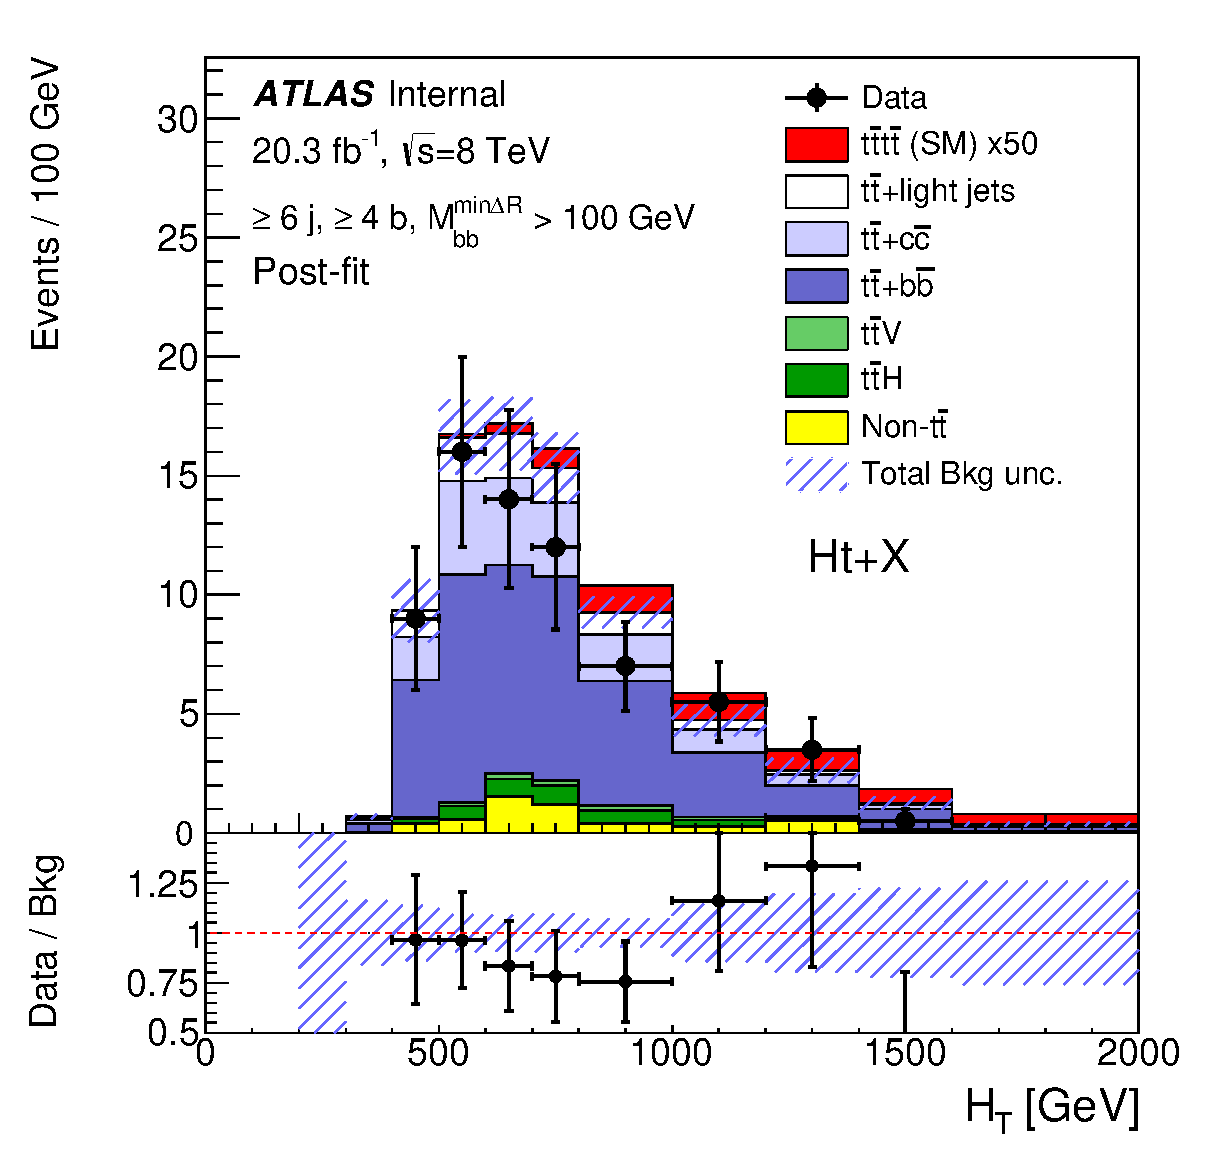
\includegraphics[width=0.49\textwidth]{Analysis/Figures_HtX/4topSM_HTAll_6jetin4btaginInHmv18TeV.eps}
  \includegraphics[width=0.49\textwidth]{Analysis/Figures_HtX/4topBSM_HTAll_6jetin4btaginInHmv18TeV.eps} \\
  \includegraphics[width=0.49\textwidth]{Analysis/Figures_HtX/Sgluon800_HTAll_6jetin4btaginInHmv18TeV.eps}
  \includegraphics[width=0.49\textwidth]{Analysis/Figures_HtX/UED800_HTAll_6jetin4btaginInHmv18TeV.eps}
  \caption{Comparison between data and prediction for the $\HT$ distribution in the most sensitive region: ($\geq$6 j, $\geq$4 b, high $M_{bb}^{{\rm min}\Delta R}$). 
The background prediction is shown after a background-only fit to data. 
Also shown is the expected signal contribution from: (a) SM \fourtop\ production scaled by a factor of 50, (b) $\fourtop$ via an EFT model with a four-top contact interaction, (c) sgluon pair production with a mass of \unit[800]{\gev}, $\fourtop$ from a model with UED and $m_{\KK} = \unit[800]{\gev}$.
The last bin in all figures contains the overflow, the hashed area represents the total uncertainty on the background and the red line represents the signal prediction normalized to the observed data.}
  \label{fig:4top_data}
\end{figure}

In the case of $\fourtop$ production with the SM kinematics, the observed (expected) 95\% CL upper limit on the
production \xsec\ is 34 (47) times the SM prediction, or \unit[23]{fb} (\unit[32]{fb}). 
In this scenario the expected sensitivity of this analysis is comparable to that of previous searches~\cite{Aad:2015gdg,Khachatryan:2014sca}.

In the case of $\fourtop$ production via an EFT model with a four-top contact interaction, the observed (expected) 95\% CL upper limit on the
production \xsec\ is \unit[12]{fb} (\unit[16]{fb}). 
The improved sensitivity in the case of the EFT model results from the harder $\HT$ spectrum compared to that of SM $\fourtop$ production.
The upper limit on the production \xsec\ can be translated into an 
observed (expected) limit on the free parameter of the model $|C_{4t}|/\Lambda^2<\unit[6.6]{\tev^{-2}}\;(\unit[7.7]{\tev^{-2}})$. 

The resulting observed and expected upper limits on the sgluon pair production \xsec\
times branching ratio are shown in figure~\ref{fig:limits_sgluon} as a function of the sgluon mass.
This translates into an observed (expected) 95\%  CL  limit  
on the sgluon mass of $1.06\tev$ ($1.02\tev$). 

Finally, the observed and expected upper limits on the production \xsec\
times branching ratio for the UED model are shown in figure~\ref{fig:limits_ued_10} as a function of $m_{\KK}$
for the symmetric case ($\xi=R_4/R_5=1$), assuming production by tier $(1,1)$ alone.
The comparison to the LO theoretical \xsec\ sets an observed (expected) 95\%  CL  limit  
on $m_{\KK}$ of $1.12\tev$ ($1.10\tev$). As discussed in section~\ref{subsubsec:KKmodes}, four-top-quark events can also arise from 
tiers $(2,0)$ and $(0,2)$. In those tiers the theoretical production \xsecs\ can be 
computed without the need to to make an assumption on the branching ratio. 
The dependence of the tier kinematics on the tier mass also allows the extrapolation of constraints on tier $(1,1)$ to tiers $(2,0)$ and $(0,2)$. 
Excluding a given production \xsec\ for tier $(1,1)$ at a given $m_{\KK}$ is equivalent to
excluding this production \xsec\ for tier $(2,0)$ alone at $m_{\KK}/\sqrt{2}$ and for tier $(0,2)$ at $m_{\KK}/\sqrt{2}\xi$. 
The contribution of tier $(0,2)$ vanishes as $\xi$ increases (highly-asymmetric case).
Figure~\ref{fig:limits_ued_20} presents the observed and expected upper limits on the production \xsec\ 
times branching ratio as  function of $m_{\KK}$ for two scenarios: tiers $(2,0)$+$(0,2)$ alone in the symmetric case,
and tier $(2,0)$ alone in the highly-asymmetric case.  In both cases a branching ratio of $A^{(1,1)}\to t\bar{t}$ of 0\% is assumed, so that only direct decays from the level-2 modes contribute to the \fourtop\ final state.
The corresponding observed (expected) 95\%  CL  limits on $m_{\KK}$ are $0.61\tev$ ($0.60\tev$) and $0.57\tev$ ($0.55\tev$) respectively. 

CMS has published results in the search for SM four-top-quark production in the lepton+jets final state~\cite{Khachatryan:2014sca}, with an expected sensitivity of \unit[32]{fb}, comparable to the presented analysis.
ATLAS has also published limits on four-top-quark production, with a search in the same-sign dilepton final state~\cite{Aad:2015gdg}. The expected limit for SM four-top production is \unit[27]{fb}, achieving a better sensitivity. However, the expected limits obtained for new physics scenarios are slightly weaker than for the presented analysis: $|C_{4t}|/\Lambda^2<\unit[9.1]{\tev^{-2}}$, $m_{\rm sgluon} < \unit[0.94]{\tev}$ and $m_{\KK} < \unit[1.05]{\tev}$. The observed limits are significantly weaker since an excess of events is observed.

The search presented here obtains the most restrictive limits to date for four-top-quark production in the various new physics scenarios considered.

\begin{figure}[tbp]
\centering
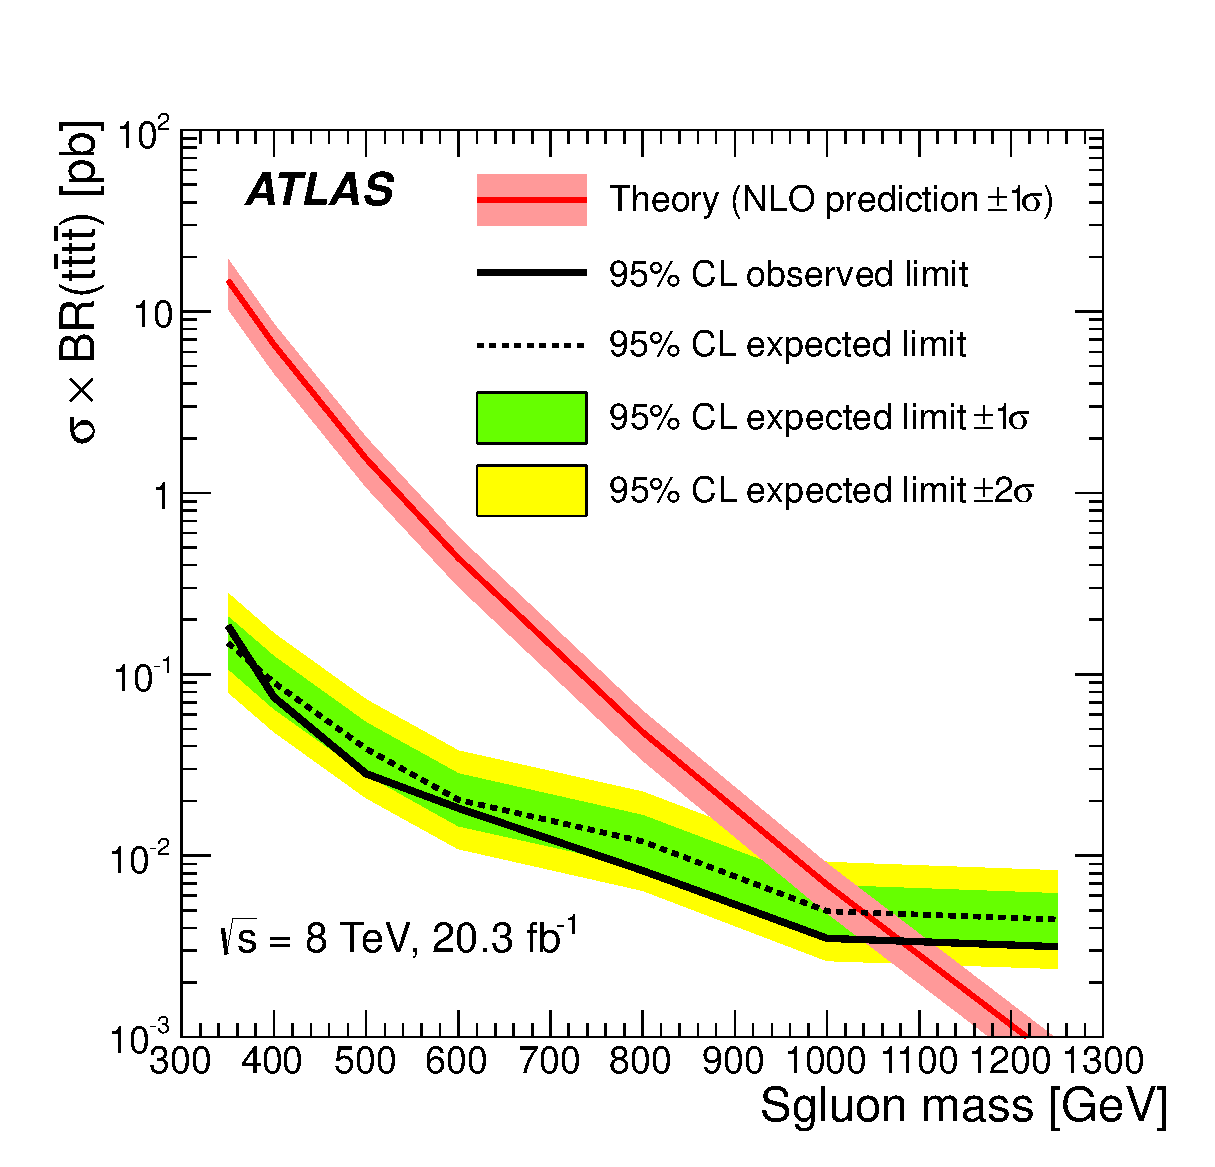
\includegraphics[width=0.45\textwidth]{Analysis/Figures_HtX/HtXPaper/Limits/lim_sgluon.eps}
\caption{
Observed (solid line) and expected (dashed line) 95\% CL upper limits on the sgluon pair production \xsec\ times 
branching ratio as a function of the sgluon mass. 
The surrounding shaded bands correspond to $\pm1$ and $\pm2$ standard deviations around the expected limit. 
The thin red line and band show the theoretical prediction and its $\pm1$ standard deviation uncertainty.
\label{fig:limits_sgluon}}
\end{figure}
\begin{figure}[tbp]
\centering
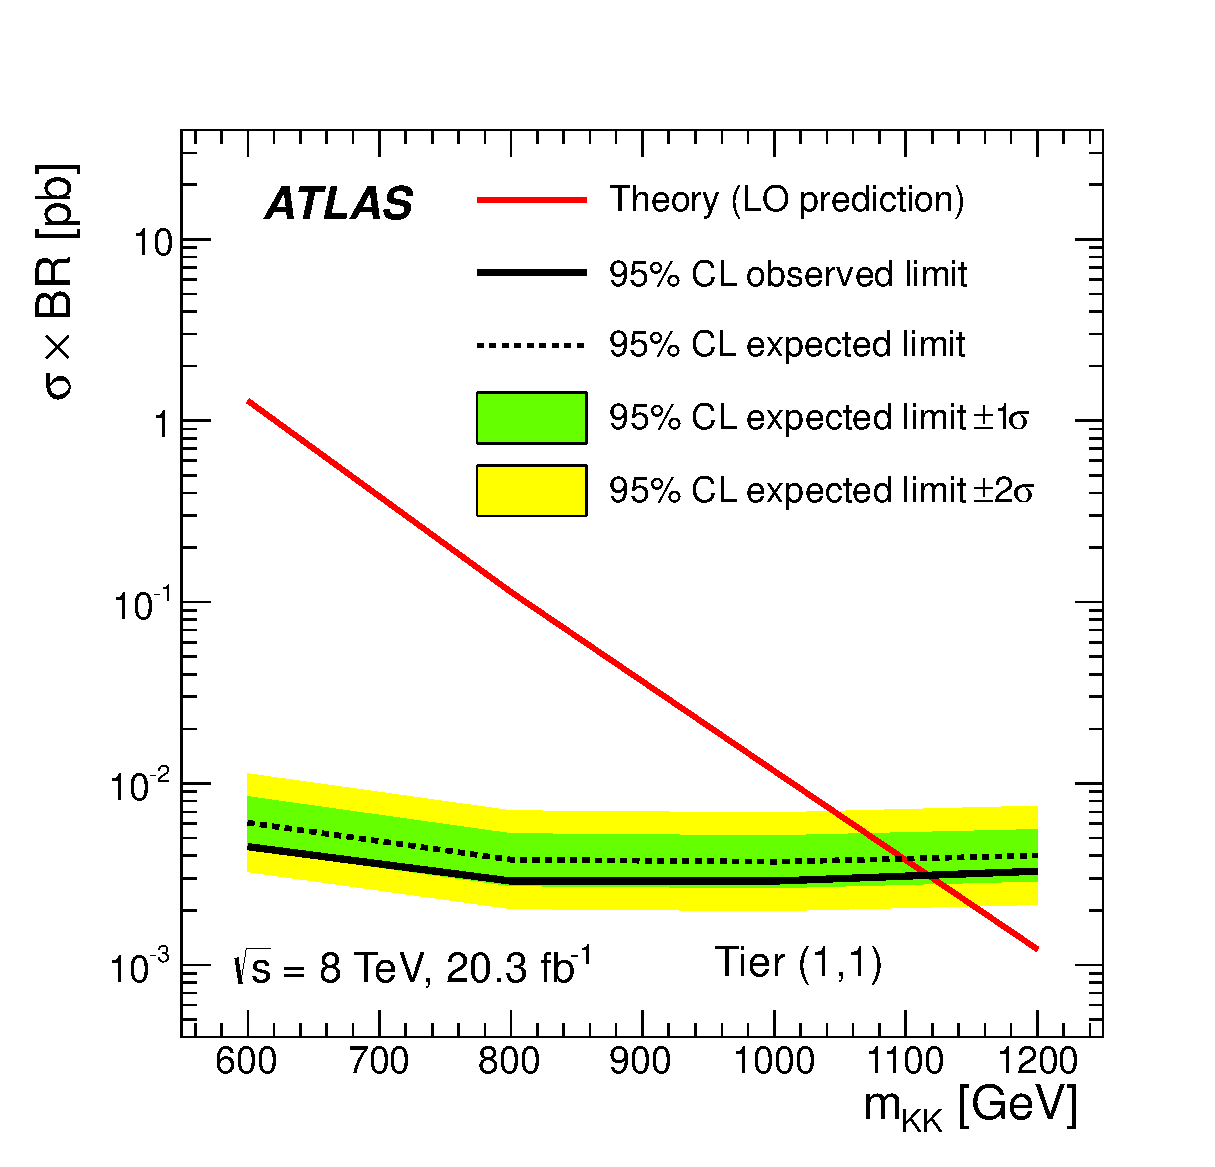
\includegraphics[width=0.45\textwidth]{Analysis/Figures_HtX/HtXPaper/Limits/lim_ued.eps}
\caption{
Observed (solid line) and expected (dashed line) 95\% CL upper limits on the production \xsec\ times branching ratio
of four-top-quark events as a function of Kaluza-Klein mass ($m_{\KK}$) from tier $(1,1)$ in the symmetric case. 
The surrounding shaded bands correspond to $\pm1$ and $\pm2$ standard deviations around the expected limit. 
The thin red line shows the theoretical prediction for the production \xsec\ of four-top-quark events by 
tier $(1,1)$ assuming BR$(A^{(1,1)}\to t\bar{t})=1$, where $A^{(1,1)}$ is the lightest particle of this tier.
\label{fig:limits_ued_10}}
\end{figure}
\begin{figure}[tbp]
\centering
\includegraphics[width=0.45\textwidth]{Analysis/Figures_HtX/HtXPaper/Limits/lim_ued_tier20_02.eps}
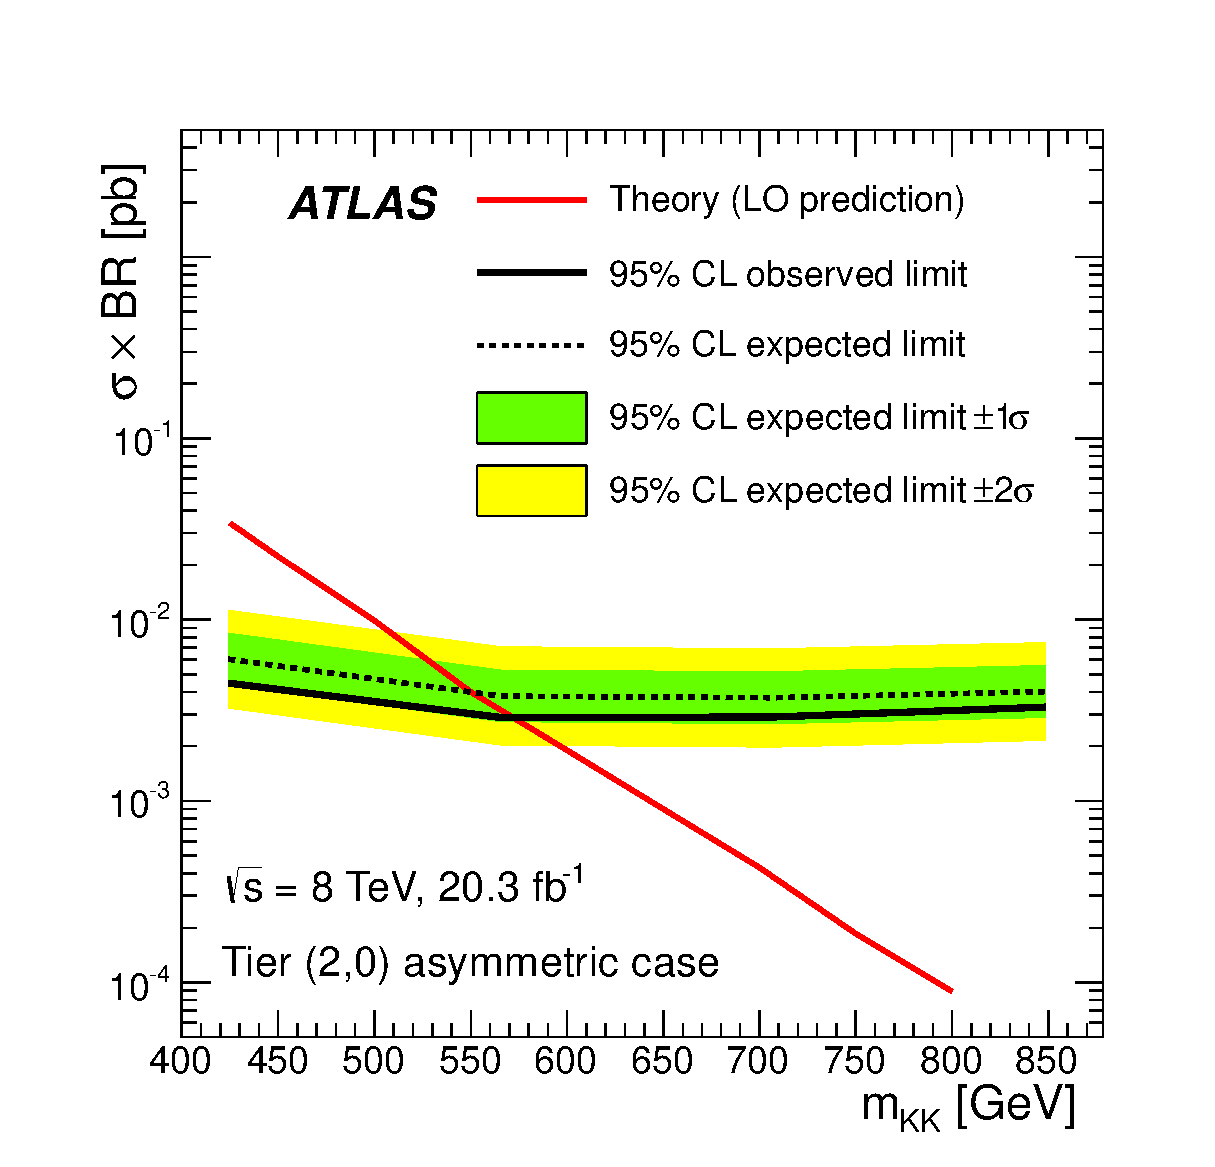
\includegraphics[width=0.45\textwidth]{Analysis/Figures_HtX/HtXPaper/Limits/lim_ued_tier20_asym.eps}
\caption{
Observed (solid line) and expected (dashed line) 95\% CL upper limits on the production \xsec\ times branching ratio
of four-top-quark events as a function of Kaluza-Klein mass ($m_{\KK}$) from (left) tiers $(2,0)$+$(0,2)$ alone in the symmetric case 
and (right) tier $(2,0)$ alone in the highly-asymmetric case.
The surrounding shaded bands correspond to $\pm1$ and $\pm2$ standard deviations around the expected limit. 
The thin red line shows the theoretical prediction for the production \xsec\ of four-top-quark events.
% and the band denotes its $\pm1$ standard deviation uncertainty.
\label{fig:limits_ued_20}}
\end{figure}

\clearpage
